\documentclass[a4paper, 11pt]{article}

\usepackage{graphicx}
\usepackage{amsmath,amssymb,amsfonts,amscd,amsthm}
\usepackage[round]{natbib}
\usepackage{wasysym}
\usepackage{booktabs}
\usepackage{setspace}
\doublespacing

\usepackage{lineno}
 \linenumbers*[1]

\title{\textbf{Forecasting atmospheric radiocarbon decline to pre-bomb values}}
\author{Carlos A. Sierra}
\date{}
%\affil{1}{Max Planck Institute for Biogeochemistry, Hans-Kn\"oll-Stra\ss e 10, 07745 Jena, Germany. Email: csierra@bgc-jena.mpg.de}

\begin{document}

\maketitle

\vspace{2cm}

\noindent
\textbf{Affiliation}:\\
{\it Max Planck Institute for Biogeochemistry, Jena, Germany}

\vspace{2cm}

\noindent
\textbf{Correspondence}: \\ Max-Planck-Institute for Biogeochemistry, Hans-Kn\"{o}ll-Str. 10, 07745 Jena, Germany. Phone: +49 3641 576133, fax: +49 3641 577100, email: csierra@bgc-jena.mpg.de.

\newpage

\begin{abstract}
In this manuscript, I present an estimation of the rate of decline in atmospheric radiocarbon and the amplitude of its seasonal cycle for the past four decades for the northern and southern hemispheres, and forecast the time required to reach pre-1950 levels (i.e. $\Delta^{14}$C $< 0 \permil$). Using a set of 30 different exponential smoothing state-space models, the time series were decomposed into their error, trend, and seasonal components, choosing the model that best represented the observed data. 
According to the best model, the rate of change in $\Delta^{14}$C has decreased considerably since the 1970s and reached values below -5 \permil \ per year since 2005. Overall, the time-series showed larger rates of radiocarbon decline in the northern than in the southern hemisphere, and relatively stable seasonal cycles for both hemispheres. A forecast of the exponential smoothing models predicts that radiocarbon values will reach pre-1950 levels by 2021 in the northern hemisphere with  20\% probability, and by around 2035 in the southern hemisphere. However, at regional levels radiocarbon concentrations have already reached pre-1950 levels in several industrialized regions and cities around the world as a consequence of fossil-fuel emissions.
\end{abstract}

\textbf{Keywords:} Time series decomposition, bomb curve, fossil fuels, cities, statistical forecast.

\newpage

%% !TEX root = Radiocarbon.tex

\section{Introduction}
In the early 1950s Hans Suess described a significant decrease in the radiocarbon content of the atmosphere due to the combustion of fossil fuels, which contain virtually no radiocarbon and therefore dilute atmospheric $^{14}$C relative to $^{12}$C \citep{Suess1953, Suess1955Sci}. This trend changed dramatically in the late 1950s and early 1960s when nuclear-bomb tests increased atmospheric radiocarbon content to levels not ever seen before in the last 50,000 years of Earth's history. Since then, radiocarbon content have been declining globally as evidenced by data from tree-rings and more recent direct atmospheric observations \citep{Tans1979Nature, Manning1990, Levin1989Radiocarbon, Currie2011, Graven2012JGR, Hua2013Radiocarbon, Levin2013Tellus}.

Using a simple box model of the global carbon cycle, \citet{Caldeira1998GRL} predicted that atmospheric radiocarbon content will continue a negative rate of decline until the beginning of the 21st century and will return to pre-1950 values around the year 2020. More recently, \citet{Graven2015PNAS} predicted a similar time for returning to pre-1950s values, but with different trajectories according to different fossil-fuel emission scenarios. This point, where $\Delta^{14}$C values go from positive to negative, indicate a transition where fossil-fuel derived CO$_2$ dominates the atmospheric signal of radiocarbon, previously dominated by bomb-derived radiocarbon. 

Determining this transition point in atmospheric radiocarbon is important for different reasons. For instance, a) it helps to determine the impact of fossil fuel emissions on the global carbon cycle \citep{Caldeira1998GRL, Turnbull2009JGR, Graven2015PNAS}, b) it serves as an important benchmark for global carbon models since the rate of radiocarbon decline is the result of different processes rates in global C reservoirs, and appropriate representation of these processes in models must predict accurately this transition point \citep{Oeschger1975Tellus, Randerson2002GBC, Naegler2006}, and c) it sets a new reference point for dating organic material of interest in biology, biogeochemistry, forensics and archeology \citep{Graven2015PNAS}. 

Post-bomb atmospheric radiocarbon data for different hemispheric zones have been compiled and homogenized  by \cite{Hua2013Radiocarbon}, harmonizing measurements from tree-rings \citep[e.g.][]{Hertelendi1983, Levin1997, Hua2000, Park2002, Yamada2005, Hua2012GRL, Rakowski2013} and direct atmospheric observations \citep[e.g.][]{Vogel1971, Berger1987, Manning1990, Nydal1996, Levin2004, Meijer2006, Turnbull2007, Levin2010Tellus, Currie2011, Graven2012JGR} (Figure \ref{fig:HuaSeries}). These hemispheric `bomb curves' contain very useful information on the trend and seasonality of atmospheric radiocarbon for different hemispheric regions. Furthermore, this information can be used to forecast future trends in atmospheric radiocarbon and determine the possible transition date to pre-1950 levels.

%Previous analysis using radiocarbon in CO$_2$ from individual stations, have shown important inter-hemispheric differences in the trend and seasonality of $\Delta^{14}$C values, helping to identify contributions from the main global sources and sinks of carbon, as well as helping to determine the strength of the interhemispheric gradient \citep{Levin2010Tellus, Graven2012JGR}. 

Compiled atmospheric radiocarbon curves are only released to the scientific community at irregular intervals \citep{Hua2004, Hua2013Radiocarbon}, and there is a need to produce forecasts of these curves for periods not covered by the compiled curves. For instance, radiocarbon dating methods or analyses of cycling rates in carbon reservoirs using samples from recently collected material require best estimates 
of the atmospheric radiocarbon values for time intervals after the latests release of the compiled radiocarbon curves \citep{SierraGMD14} . For this reason, it is important to provide robust statistical methods for forecasting that can provide accurate predictions. 

Here I present a time-series decomposition analysis for the atmospheric radiocarbon curves of \citet{Hua2013Radiocarbon}, fitting a set of exponential smoothing state-space models with the aim to forecast future trends in radiocarbon at hemispheric scales. The main objectives of this analysis are, a) to decompose the observed time series into trend and seasonal components and characterize differences among hemispheric zones, and b) to identify the probability of returning to pre-bomb radiocarbon values; i.e. $\Delta^{14}$C $\leq 0 \permil$. Additionally, I present radiocarbon measurements of plants from different cities to identify the degree at which, by local dilution, atmospheric radiocarbon has already crossed this threshold. 

%\begin{figure}[htbp]
%   \centering
%   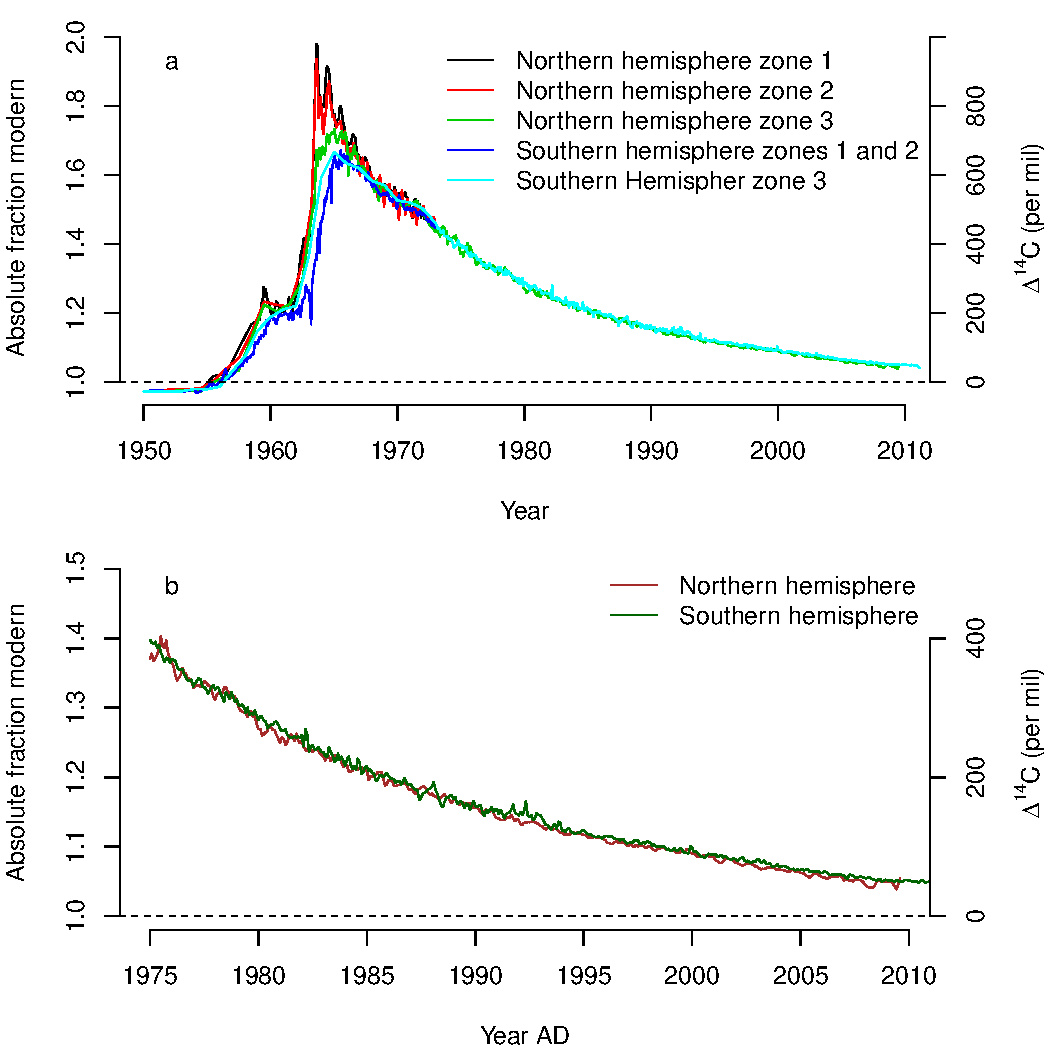
\includegraphics[scale=0.7]{Figures/HuaSeries} % requires the graphicx package
%   \caption{Atmospheric radiocarbon for four atmospheric regions. a) Original data from \citet{Hua2013Radiocarbon}, b) time series constructed from original data for the period 1975 to 2010.}
%   \label{fig:HuaSeries}
%\end{figure}


\section{Methods}
\subsection{Time series decomposition} 
I used the harmonized atmospheric radiocarbon time series reported by \citet{Hua2013Radiocarbon} for the northern and southern hemispheres. Although these authors present curves for four different hemispheric zones, the curves only deviate from each other during
the early bomb period. Here, I used data from the year 1975 to 2010, where intra-hemispheric differences are not reported, and only
the northern and the southern hemispheres are differentiated. 

These hemispheric radiocarbon time-series are not available at regularly spaced intervals as required by the time-series analysis used here; therefore, they were homogenized in regular monthly and seasonal periods by cubic spline interpolation (Figure \ref{fig:HuaSeries}b).

To analyze each time series, I used the ETS framework described by \citet{Hyndman2008} to fit 30 different exponential smoothing state-space models that decompose the series in the error (E), trend (T), and seasonal (S) components (ETS decomposition). In classical time-series decomposition methods, trend, seasonality and error are commonly assumed as linear additive terms \citep[e.g.][]{Cleveland1983}, which in the ETS framework imply a model of the form E+T+S. However, many other methods have been proposed to decompose time series in its inherent components, not only considering linear additive models. For instance, models can have all terms multiplicative (E*T*S), or combinations between additive and multiplicative terms (e.g. E*T+S). The different combinations of potential model structures results in the 30 different models tested here. As selection criterion, I used the Akaike information criterion (AIC), which selects the best model according to goodness of fit and the complexity of the model, given preference to the simplest model that can best predict the observations. 

When the data contains zeros or negative values, the multiplicative error models in the ETS framework are not numerically stable \citep{Hyndman2008}. For this reason, I used the radiocarbon series as \emph{absolute fraction modern} $F'$ in all computations \citep{Trumbore2016}, which expresses $\Delta^{14}$C values as a fraction by the relation

\begin{equation}
\Delta^{14} \text{C} = (F' -1) \cdot 1000,
\end{equation}
and can also be interpreted as fraction modern $F$ corrected for radioactive decay of the OX1 standard since 1950. More precisely, 

\begin{equation}
F' = F \cdot \exp((1950-x)/8267),
\end{equation}
where $x$ is the year of sample collection and measurement. 


ETS models predict observations $y_t$ according to a function of the error, trend, and seasonal components $f(E, T, S)$. The trend component is also split between a level $l$ and a growth term $b$. The error term $\varepsilon$ is considered a Gaussian white-noise process with variance $\sigma^2$. The mean value of the observations is therefore predicted by a function

\begin{equation}
\mu_t = f(l, b, s, \theta),
\end{equation}
where $s$ is the seasonal trend and $\theta$ are a set of constant parameters that weigh the contributions from the different components. Parameter estimation is performed by 
maximum likelihood. 

Forecasting is performed by recursively applying the ETS model $h$ number of steps ahead the last observation. Specific details about the method and its implementation in the R package {\tt forecast} are provided in \citet{Hyndman2008} and \citet{Hyndman2008JSS}, respectively. In the supplementary material I provide all code necessary to reproduce the results presented here.

\subsection{Radiocarbon in local air}
I also used radiocarbon analyses of annual plants to infer the atmospheric radiocarbon concentration in a set of cities around the world. Annual plants incorporate local sources of carbon dioxide during the growing season, providing an integrated measure of the radiocarbon concentration of the local air \citep{Hsueh2007GRL}. For consistency, I sampled at each location at least three individuals of dandelion ({\it Taraxacum spp.}), an annual plant that can be found growing in most cities. For comparison, I also sampled plants at locations with low influence of anthropogenic fossil fuel emissions such as the Rocky Mountain National Park (RMNP) in the USA, the Austrian Alps, and in the Amazon basin at the town of Leticia, Colombia. Plants were washed and air-dried after sampling to eliminate contamination from dust and other particles.   All samples were then oven-dried at 70$^{\circ}$ Celsius and ground in a ball-grinder at the Max Planck Institute for Biogeochemistry in Jena, Germany. Radiocarbon analyses were conducted by Accelerator Mass Spectrometry at the same institution \citep{Steinhof2004Radiocarbon}. 

\section{Results}
\subsection{Time series decomposition}
From the 30 different competing models, the best performance was obtained by an ETS model of the form: (M,A,M), which means that the 
error and the seasonal terms are multiplicative, and the trend term is additive. Specifically, for both hemispheric curves the model with
the best AIC had the form:

\begin{align}
\mu_t &= (l_{t-1} + b_{t-1}) s_{t-m}, \notag \\
l_t &= (l_{t-1} + b_{t-1}) (1 + \alpha \varepsilon_t), \notag \\
b_t &= b_{t-1} + \beta (l_{t-1} + b_{t-1})\varepsilon_t , \notag \\
s_t &= s_{t-m} (1+ \gamma \varepsilon_t), \notag
\end{align}
where $\alpha$, $\beta$, and $\gamma$ are constant parameters, and  the $t-m$ subscript represents the intra-annual time-step that composes the seasonal cycle of the seasonal term $s$. 

For the northern hemisphere time series, the value of the parameters were $\theta_{NH}: (\alpha = 0.7551, \beta = 0.0346, \gamma = 0.0001)$; and for the southern hemisphere $\theta_{SH} : (\alpha = 0.2504, \beta = 0.0086, \gamma = 0.0001)$. Notice that the main differences among the two models are on the parameters $\alpha$ and $\beta$ that control the degree by which the error term influence the level and growth terms, respectively. This implies that for the northern hemisphere, the level and the growth terms showed more variability than in the southern hemispheres (Figure \ref{fig:SlopeSeason}). The seasonal term had very little influence from the error term as predicted by  $\gamma$, therefore the seasonal cycle obtained from this model had a very regular pattern. 

The temporal pattern of the growth term $b_t$ was relatively similar between the northern and the southern hemispheres (Figure \ref{fig:SlopeSeason}b), but the curve for the level term was always lower for the northern hemisphere, which results in a larger decline of atmospheric radiocarbon for the north (Figure \ref{fig:SlopeSeason}a). For the last years in both time series, from 2005 to 2011,
the annual decline in atmospheric radiocarbon in $\Delta^{14}$C was below -5 $\permil$ in both hemispheres, but with relatively high uncertainty  as  accounted by the $\varepsilon$ term (Table \ref{tab:slopes}).


Since the seasonal pattern is a multiplicative term centered around 1, the absolute amplitude of the seasonal cycle is predicted to decline in this model for both hemispheres, but proportionally to the actual radiocarbon concentration in the atmosphere. The lower the value of the trend ($l + b$) the lower the amplitude of the term $\mu_t$. The model predicts a higher influence of the seasonal term for the northern than for the southern hemisphere.
The model also predicts, as previously reported \citep{Levin2010Tellus, Currie2011}, a reversed seasonality between the northern and the southern hemispheres (Figure \ref{fig:SlopeSeason}c). 

%\begin{figure}[htbp]
%   \centering
%   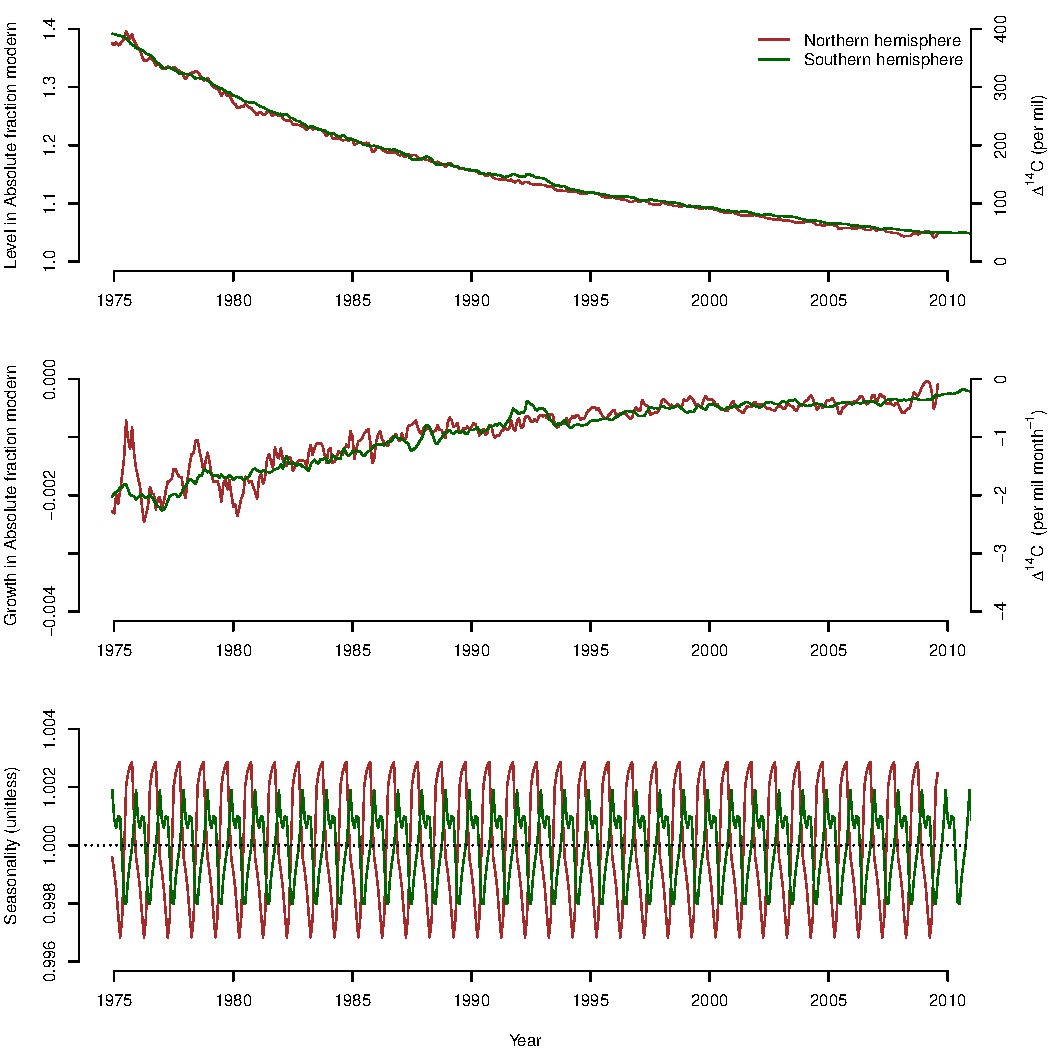
\includegraphics[scale=0.7]{Figures/SlopeSeason} % requires the graphicx package
%   \caption{Trend (level and slope) and seasonality of the atmospheric radiocarbon time series predicted by the best-fit model for the hemispheric series compiled by \citet{Hua2013Radiocarbon}. For both series the best model selected based on the AIC was an ETS model of the form (M,A,M), i.e. a multiplicative term for the error, an additive term for the trend, and a multiplicative term for the seasonality. }
%   \label{fig:SlopeSeason}
%\end{figure}
%
\subsection{Forecast}
A forecast of the atmospheric radiocarbon time series was obtained by exponential smoothing of the ETS model, i.e. recursively applying the set of equations with the best parameter values found \citep{Hyndman2008}. The forecast was obtained on quarterly intervals and not on a monthly basis since the multiplicative error term strongly influences uncertainty bounds in predictions at short-time scales. This is a relatively well-known issue in forecasting methods \citep{Athanasopoulos}, and it is commonly recommended to produce forecasts at an intermediate time-scale such as every four months in long-term monthly time-series \citep{Nijman1990, Rossana1995, Athanasopoulos}. 

For the two series, the forecast of the average radiocarbon values showed a linear decrease for the next 20 years (Figure \ref{fig:Forecast}). This linear decline is based on the observed stabilization of the growth term of the time series (Figure \ref{fig:SlopeSeason}a). The range of the prediction intervals increases in all series because of the nature of the exponential smoothing model that assigns less weight to successively older observations and therefore the uncertainty in the predictions increases. 

Atmospheric radiocarbon is predicted to decline faster in the northern hemisphere than in the southern hemisphere, therefore it is more likely that radiocarbon values return to pre-1950 values earlier in the northern hemisphere. Uncertainty ranges are also higher for the northern than for the southern hemisphere as a consequence of higher values of the parameters $\alpha$ and $\beta$ from the ETS model.

Independent observations of atmospheric radiocarbon from European stations at the Schauinsland and Jungfraujoch sites \citep{Levin2013Tellus}, are within forecast uncertainty range for the northern hemisphere (Figure \ref{fig:ForecastEurope}a). The observations from Jungfraujoch follow relatively well the forecasted mean and the seasonal cycle; however for Schauinsland, the independent observations are below the forecasted mean. 
One likely explanation for this difference in the Schauinsland station, is the potential contribution of fossil-fuel derived carbon from the nearby city of Freiburg, Germany \citep{Levin1989Radiocarbon, Turnbull2009JGR, Levin2013Tellus}.

%\begin{figure}[htbp]
%   \centering
%   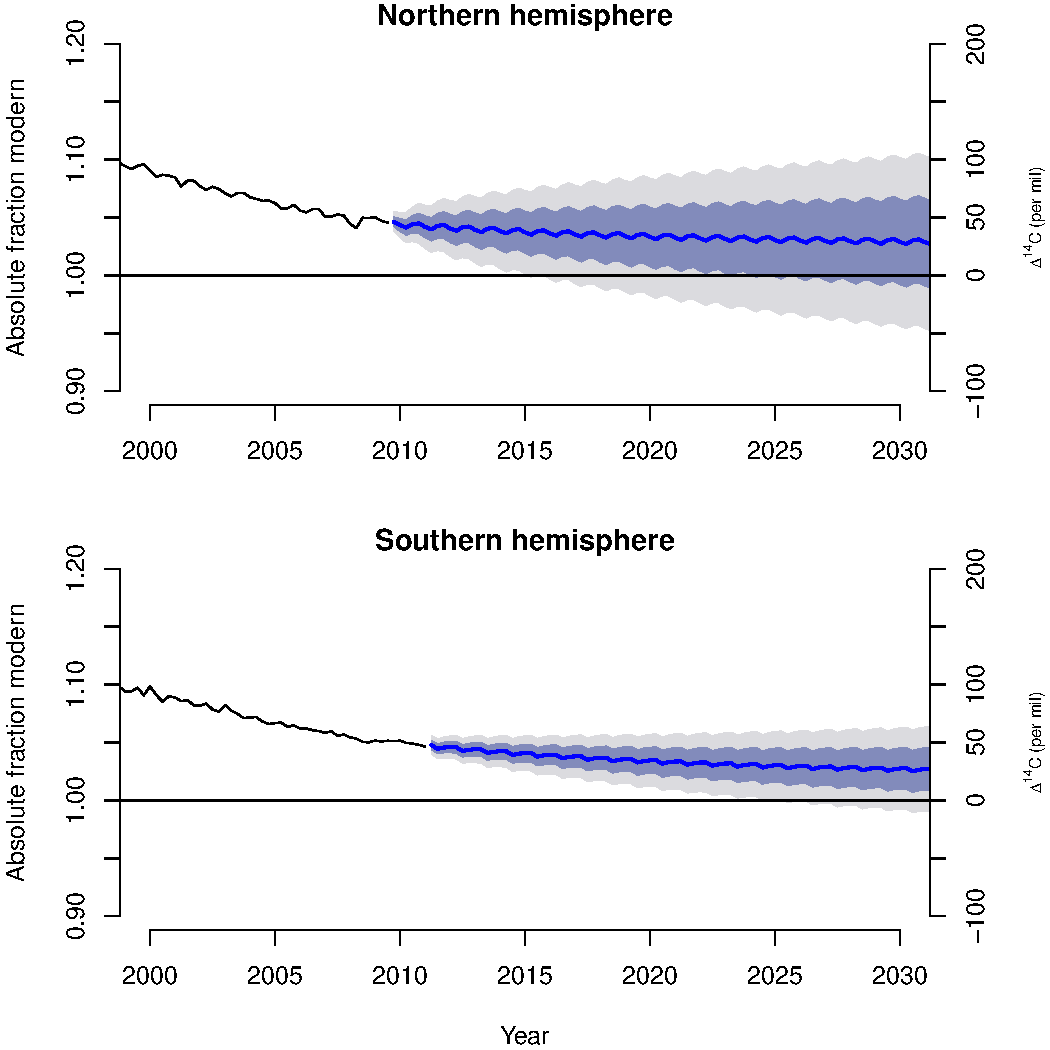
\includegraphics[scale=0.7]{Figures/Forecast} % requires the graphicx package
%   \caption{Forecast of atmospheric radiocarbon for the northern and southern hemispheres based on the best ETS model. Shaded regions in gray and blue show the 95 and 80\% prediction intervals. }
%   \label{fig:Forecast}
%\end{figure}

To predict the decline in atmospheric radiocarbon for central Europe based on the Jungfraujoch and Schauinsland stations, I ran a forecast selecting the ETS model that best matches the observations reported in \citet{Levin2013Tellus} (Figure \ref{fig:ForecastEurope}b). In this forecast, the rate of radiocarbon decline is faster, and mean atmospheric radiocarbon crosses the $\Delta^{14}$C = 0 $\permil$ threshold much earlier.

%\begin{figure}[htbp]
%   \centering
%   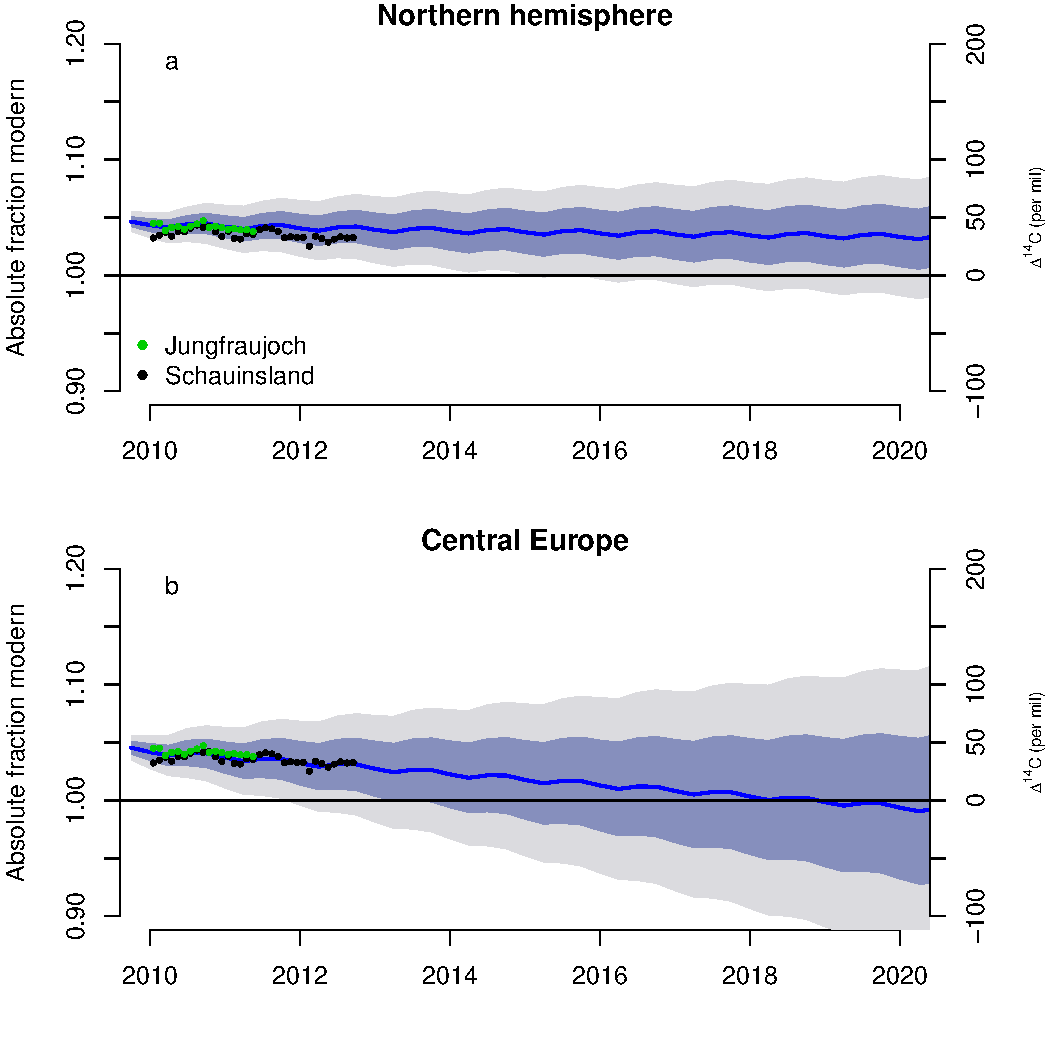
\includegraphics[scale=0.7]{Figures/ForecastEurope} % requires the graphicx package
%   \caption{a) Forecast (with 80 and 95\% prediction intervals) for the northern hemisphere radiocarbon curve compared to observations at the Jungfraujoch and Schauinsland reported in \citet{Levin2013Tellus}. b) Optimized forecast for central Europe forcing the model to pass through the observations from these two stations.}
%   \label{fig:ForecastEurope}
%\end{figure}

Atmospheric radiocarbon is expected to return to pre-1950s levels within the next decades with different probabilities for the different hemispheres. Values of $\Delta^{14}$C $\leq 0 \permil$ are within 95\% prediction intervals of the forecast starting as early as 2016 for the northern hemisphere, and 2025 for the southern hemisphere. For central Europe, it is very likely ($> 90$\% probability) that the $\Delta^{14}$C $\leq 0 \permil$ threshold is being crossed by summer 2018.


%\begin{figure}[htbp]
%   \centering
%   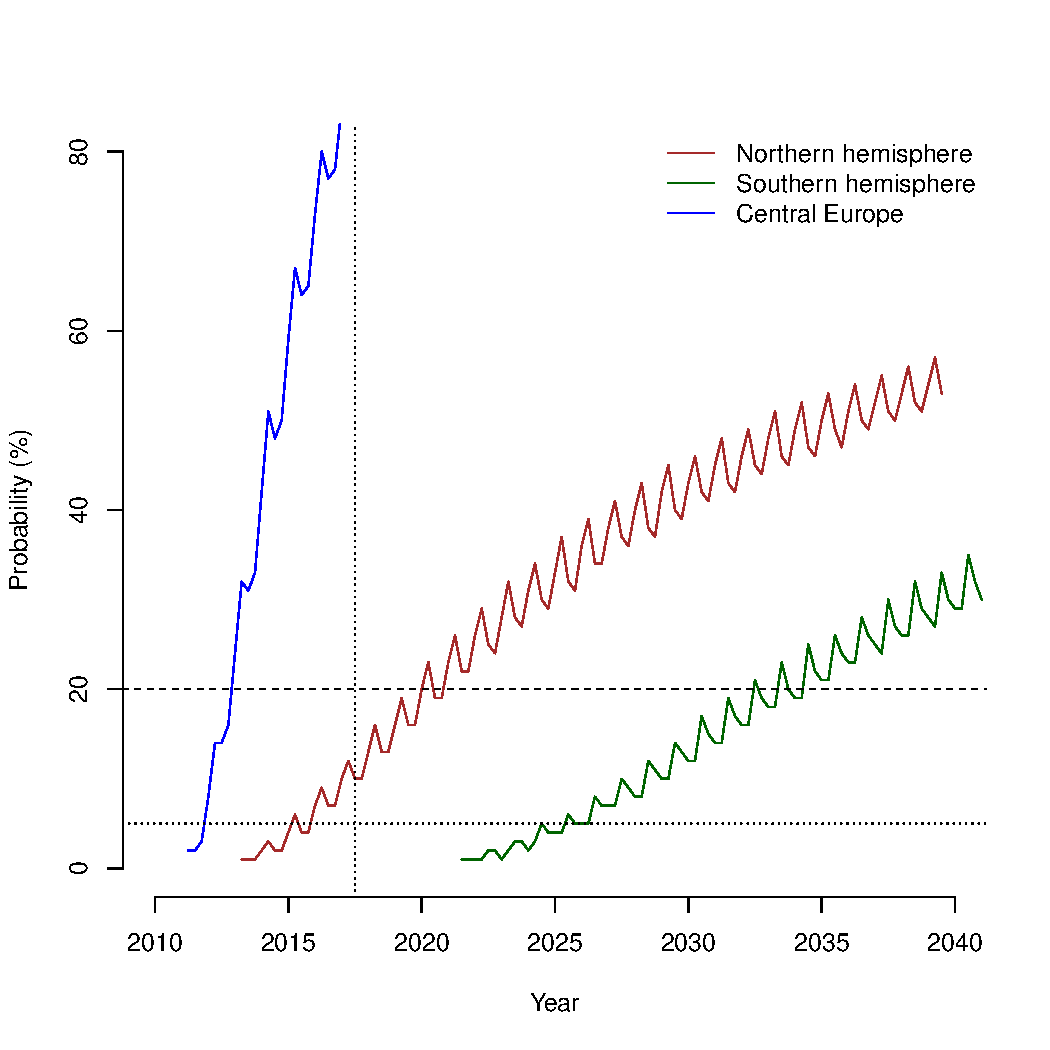
\includegraphics[scale=0.7]{Figures/Prob} % requires the graphicx package
%   \caption{Probability of $\Delta^{14}$C $\leq 0 \permil$ for the different hemispheric zones calculated as 100 minus different probability levels of the lower prediction interval for each forecast time. As a reference, 20 and 5\% probability levels are presented in dashed and dotted lines, respectively.}
%   \label{fig:Prob}
%\end{figure}

Although the hemispheric averages of background air are expected to return to pre-1950 levels within the next decades, this threshold has been already crossed locally in major cities around the world (Figure \ref{fig:Cities}, Table \ref{tab:cities}). Air in metropolitan areas with high fossil-fuel emission levels such as Medell\'in, Stockholm, and the Newport Beach area in California show the highest influence of fossil-fuel derived carbon. 
Air in European cities such as Berlin and Prague had not crossed the pre-1950 level yet, but Jerusalem was in the limit in 2014 ($-0.1 \pm 2.4$ \permil). As expected, the high altitude samples from the Austrian Alps are very close to the forecasted global values, whereas the samples from Rocky Mountain National Park were much below the forecasted global average, but within the 95\% prediction interval of the forecast.

%\begin{figure}[htbp]
%   \centering
%   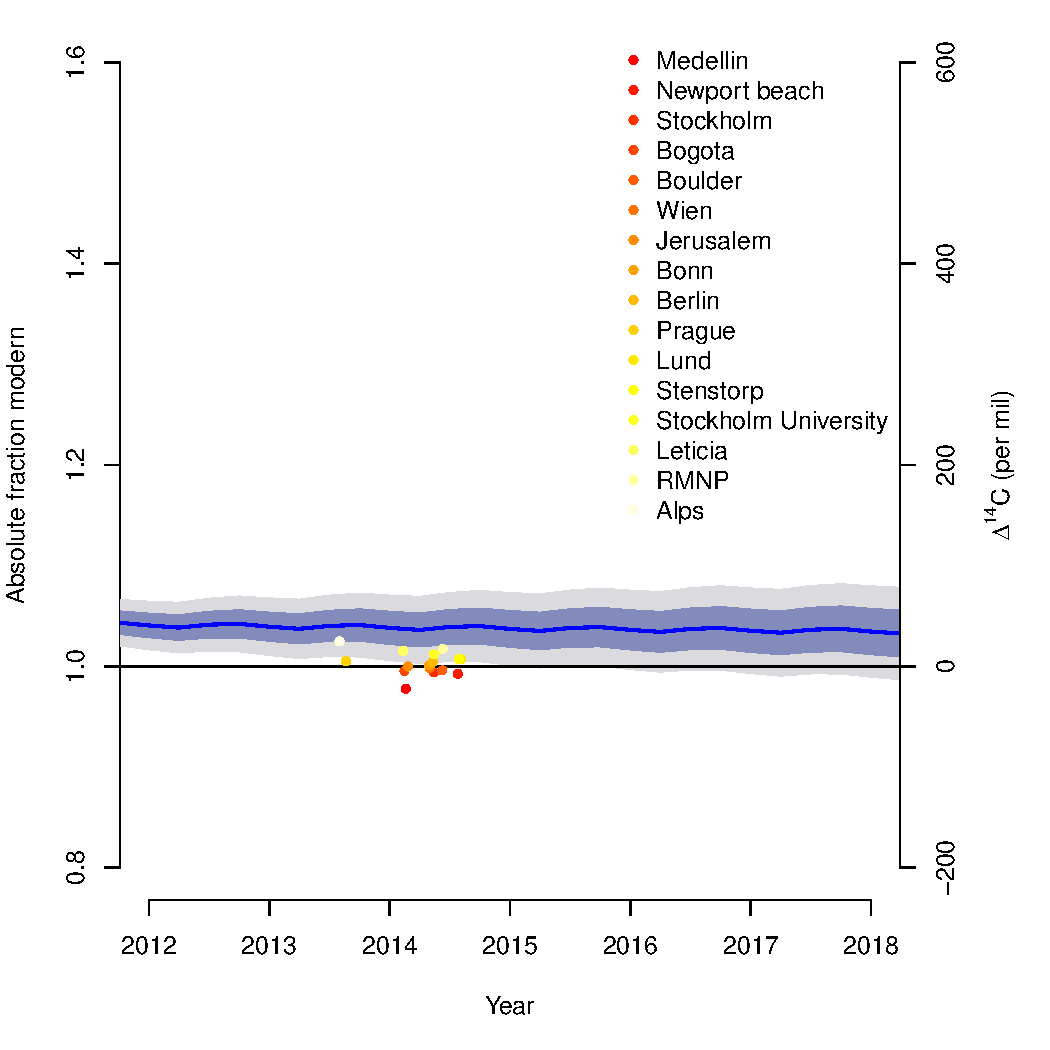
\includegraphics[scale=0.7]{Figures/Cities} % requires the graphicx package
%   \caption{Forecasted northern hemisphere atmospheric radiocarbon concentrations (with 80 and 95\% prediction intervals), based on data from \citet{Hua2013Radiocarbon}, superimposed with radiocarbon concentration measured in plants growing on different industrial cities and remote areas without fossil fuel influence. This radiocarbon concentration represents the mix of fossil-fuel derived carbon and the mixing with background air. }
%   \label{fig:Cities}
%\end{figure}


\section{Discussion}
The time series decomposition presented here shows properties of the trend, slope, and seasonality of atmospheric radiocarbon for different hemispheric zones that complements previous analyses based on sets of individual stations \citep{Levin2010Tellus, Graven2012JGR, Levin2013Tellus} and global carbon models \citep{Caldeira1998GRL, Randerson2002GBC, Turnbull2009JGR, Levin2010Tellus, Graven2015PNAS}. One main advantage of this analysis is the use of the harmonized series compiled by \citet{Hua2013Radiocarbon}, which provide a spatial average across the different stations from which atmospheric radiocarbon has been measured. The series also resolve issues of temporal gaps for the individual stations, and give a comprehensive overview of the dynamic behavior of atmospheric radiocarbon in background air during the past 40 years for the two hemispheres. 

The series decomposition analyses showed that the overall decline of atmospheric radiocarbon was higher in the northern hemisphere than in the southern hemisphere. This is not surprising because the large levels of fossil-fuel emissions in the northern hemisphere are expected to significantly dilute atmospheric radiocarbon \citep{Levin1989Radiocarbon, Levin2010Tellus, Turnbull2009JGR, Graven2012JGR}. Rates of decline since 2005 have been below $ -5 \permil$ per year. This implies that if rates of decline continue decreasing, they may pose significant challenges for detecting annual trends in atmospheric radiocarbon given that the uncertainty in new generation AMS systems is between 3 to 2$\permil$ \citep{Synal2007, Wacker2010}.

Atmospheric radiocarbon is expected to return to pre-1950 levels in the northern hemisphere by 2020, the year predicted by  \citet{Caldeira1998GRL}, with a probability $\sim$20\% (Figure \ref{fig:Prob}). In the southern hemisphere however, it is unlikely that atmospheric radiocarbon reach values below 0 $\permil$ by 2020. Based on more recent observations from central Europe, the pre-1950 threshold may be crossed with high probability ($>$90\%) by summer 2018 (Figure \ref{fig:Prob}). 

It is not possible to attribute any particular process that may contribute to the observed trends in the data with this statistical approach. However, previous analyses \citep{Caldeira1998GRL, Randerson2002GBC, Levin2013Tellus, Currie2011} may help to explain some of the properties of the observed time series. For instance, different processes are responsible for determining atmospheric radiocarbon content: fossil fuel emissions, ocean-atmosphere exchange, stratosphere-troposphere mixing, terrestrial ecosystem fluxes, emissions from nuclear industry, and cosmogenic production \citep{Oeschger1975Tellus, Randerson2002GBC, Naegler2006, Levin2010Tellus, Graven2015PNAS}. The recent slower rates of decline in the northern hemisphere may be explained by the contribution of the terrestrial biosphere and oceans that return decades-old bomb radiocarbon and therefore counterbalance the effect of increased fossil fuel emissions \citep{Caldeira1998GRL, Randerson2002GBC, Currie2011}. For the southern hemisphere, ocean-atmosphere exchange plays a larger role, and the slow in radiocarbon decline in recent years may be explained by return of bomb radiocarbon by the mixed layer \citep{Currie2011}.

The combined effect of terrestrial biosphere, ocean exchange, fossil-fuel emissions as well as horizontal and vertical air transport may have an important contribution in reducing the amplitude of the seasonal cycle \citep{Levin2010Tellus}. The best ETS model identified here predicts the seasonal cycle as proportional to the trend term; i.e. the higher the amount of radiocarbon in the atmosphere the higher the amplitude of the seasonal cycle, and as radiocarbon content decline in both hemispheres so does its seasonality. Given that the growth term of the series had stabilized in the recent decade, the amplitude of the seasonal cycle had remained constant in the last part of the curve. These results are consistent with model predictions by \citet{Randerson2002GBC}, who predicted a decline in seasonality over time due to decrease in seasonality in ocean and terrestrial biosphere exchange, with strong contributions from fossil-fuel signals. 

%\citet{Randerson2002GBC} predicted a decline in the seasonality of atmospheric radiocarbon as a consequence of a time-lag in the terrestrial biosphere respiring pre-modern carbon, but the decline in seasonality occurs much faster in their model predictions than in the series decomposition presented here. One possible explanation is that mean transit times of carbon in the terrestrial biosphere are much longer than those considered by \citet{Randerson2002GBC} in their analysis. 
%Another possible explanation is that fossil-fuel emissions in the northern hemisphere consistently dilute the radiocarbon signal of the respired C from the terrestrial biosphere in the summer months depending on the phase-lag between these two processes. Alternatively, processes related to stratosphere-troposphere exchange may help to explain this decline in seasonality. These hypotheses however, require further examination.

\citet{Caldeira1998GRL}, and more recently \citet{Graven2015PNAS}, predicted that in a business-as-usual scenario of fossil-fuel emissions, radiocarbon content would return to pre-1950 levels by $\sim$2020. Current trajectories of atmospheric radiocarbon seem to agree with this prediction, but with important differences among hemispheric regions. The $\Delta^{14}$C $\leq 0 \permil$ threshold would be crossed in the northern hemisphere with higher probability than in the southern hemisphere, which may be a consequence of differences in contributions between the terrestrial biosphere and the oceans, the later being more relevant for the southern hemisphere. 
It is also likely that the rate of decline of atmospheric radiocarbon in the northern hemisphere may increase in the future (become more negative) if the previously sequestered bomb-radiocarbon is exhausted, and then fossil-fuel derived carbon may have a larger influence in the northern hemisphere. This is clearly illustrated in the urban areas we analyzed where fossil-fuel emissions dominate over terrestrial exchange  and therefore radiocarbon is close or have already crossed the $\Delta^{14}$C $\leq 0 \permil$ threshold. 

The forecasted atmospheric radiocarbon curves presented here may be useful for different studies where data on the atmospheric background is not available after the latest release of the compiled curves \citep{Hua2013Radiocarbon}. The methodology of time-series decomposition and forecast may also be useful to produce forecasts for individual stations or for new releases of compiled curves. However, care must be taken in using these forecasts in different applications, and prediction uncertainties must always be considered.
Possible changes in the rates of decline of atmospheric radiocarbon for the different hemispheres may deviate in the future from the rates calculated in the time-series decomposition presented here. Therefore, these forecasted radiocarbon trends must be used with caution.


\section{Introduction}
In the early 1950s Hans Suess described a significant decrease in the radiocarbon content of the atmosphere due to the combustion of fossil fuels, which contain virtually no radiocarbon and therefore dilute atmospheric $^{14}$C relative to $^{12}$C \citep{Suess1953, Suess1955Sci}. This trend changed dramatically in the late 1950s and early 1960s when nuclear-bomb tests increased atmospheric radiocarbon content to levels not ever seen before in the last 50,000 years of Earth's history. Since then, radiocarbon content have been declining globally as evidenced by data from tree-rings and more recent direct atmospheric observations \citep{Tans1979Nature, Manning1990, Levin1989Radiocarbon, Currie2011, Graven2012JGR, Hua2013Radiocarbon, Levin2013Tellus}.

Using a simple box model of the global carbon cycle, \citet{Caldeira1998GRL} predicted that atmospheric radiocarbon content will continue a negative rate of decline until the beginning of the 21st century and will return to pre-1950 values around the year 2020. More recently, \citet{Graven2015PNAS} predicted a similar time for returning to pre-1950s values, but with different trajectories according to different fossil-fuel emission scenarios. This point, where $\Delta^{14}$C values go from positive to negative, indicate a transition where fossil-fuel derived CO$_2$ dominates the atmospheric signal of radiocarbon, previously dominated by bomb-derived radiocarbon. 

Determining this transition point in atmospheric radiocarbon is important for different reasons. For instance, a) it helps to determine the impact of fossil fuel emissions on the global carbon cycle \citep{Caldeira1998GRL, Turnbull2009JGR, Graven2015PNAS}, b) it serves as an important benchmark for global carbon models since the rate of radiocarbon decline is the result of different processes rates in global C reservoirs, and appropriate representation of these processes in models must predict accurately this transition point \citep{Oeschger1975Tellus, Randerson2002GBC, Naegler2006}, and c) it sets a new reference point for dating organic material of interest in biology, biogeochemistry, forensics and archeology \citep{Graven2015PNAS}. 

Post-bomb atmospheric radiocarbon data for different hemispheric zones have been compiled and homogenized  by \cite{Hua2013Radiocarbon}, harmonizing measurements from tree-rings \citep[e.g.][]{Hertelendi1983, Levin1997, Hua2000, Park2002, Yamada2005, Hua2012GRL, Rakowski2013} and direct atmospheric observations \citep[e.g.][]{Vogel1971, Berger1987, Manning1990, Nydal1996, Levin2004, Meijer2006, Turnbull2007, Levin2010Tellus, Currie2011, Graven2012JGR} (Figure \ref{fig:HuaSeries}). These hemispheric `bomb curves' contain very useful information on the trend and seasonality of atmospheric radiocarbon for different hemispheric regions. Furthermore, this information can be used to forecast future trends in atmospheric radiocarbon and determine the possible transition date to pre-1950 levels.

Compiled atmospheric radiocarbon curves are only released to the scientific community at irregular intervals \citep{Hua2004, Hua2013Radiocarbon}, and there is a need to produce forecasts of these curves for periods not covered by the compiled curves. For instance, radiocarbon dating methods or analyses of cycling rates in carbon reservoirs using samples from recently collected material require best estimates 
of the atmospheric radiocarbon values for time intervals after the latests release of the compiled radiocarbon curves \citep{SierraGMD14} . For this reason, it is important to provide robust statistical methods for forecasting that can provide accurate predictions. 

Here I present a time-series decomposition analysis for the atmospheric radiocarbon curves of \citet{Hua2013Radiocarbon}, fitting a set of exponential smoothing state-space models with the aim to forecast future trends in radiocarbon at hemispheric scales. The main objectives of this analysis are, a) to decompose the observed time series into trend and seasonal components and characterize differences among hemispheric zones, and b) to identify the probability of returning to pre-bomb radiocarbon values; i.e. $\Delta^{14}$C $\leq 0 \permil$. Additionally, I present radiocarbon measurements of plants from different cities to identify the degree at which, by local dilution, atmospheric radiocarbon has already crossed this threshold. 


\section{Methods}
\subsection{Time series decomposition} 
I used the harmonized atmospheric radiocarbon time series reported by \citet{Hua2013Radiocarbon} for the northern and southern hemispheres. Although these authors present curves for four different hemispheric zones, the curves only deviate from each other during
the early bomb period. Here, I used data from the year 1975 to 2010, where intra-hemispheric differences are not reported, and only
the northern and the southern hemispheres are differentiated. 

These hemispheric radiocarbon time-series are not available at regularly spaced intervals as required by the time-series analysis used here; therefore, they were homogenized in regular monthly and seasonal periods by cubic spline interpolation (Figure \ref{fig:HuaSeries}b).

To analyze each time series, I used the ETS framework described by \citet{Hyndman2008} to fit 30 different exponential smoothing state-space models that decompose the series in the error (E), trend (T), and seasonal (S) components (ETS decomposition). In classical time-series decomposition methods, trend, seasonality and error are commonly assumed as linear additive terms \citep[e.g.][]{Cleveland1983}, which in the ETS framework imply a model of the form E+T+S. However, many other methods have been proposed to decompose time series in its inherent components, not only considering linear additive models. For instance, models can have all terms multiplicative (E*T*S), or combinations between additive and multiplicative terms (e.g. E*T+S). The different combinations of potential model structures results in the 30 different models tested here. As selection criterion, I used the Akaike information criterion (AIC), which selects the best model according to goodness of fit and the complexity of the model, given preference to the simplest model that can best predict the observations. 

When the data contains zeros or negative values, the multiplicative error models in the ETS framework are not numerically stable \citep{Hyndman2008}. For this reason, I used the radiocarbon series as \emph{absolute fraction modern} $F'$ in all computations \citep{Trumbore2016}, which expresses $\Delta^{14}$C values as a fraction by the relation

\begin{equation}
\Delta^{14} \text{C} = (F' -1) \cdot 1000,
\end{equation}
and can also be interpreted as fraction modern $F$ corrected for radioactive decay of the OX1 standard since 1950. More precisely, 

\begin{equation}
F' = F \cdot \exp((1950-x)/8267),
\end{equation}
where $x$ is the year of sample collection and measurement. 


ETS models predict observations $y_t$ according to a function of the error, trend, and seasonal components $f(E, T, S)$. The trend component is also split between a level $l$ and a growth term $b$. The error term $\varepsilon$ is considered a Gaussian white-noise process with variance $\sigma^2$. The mean value of the observations is therefore predicted by a function

\begin{equation}
\mu_t = f(l, b, s, \theta),
\end{equation}
where $s$ is the seasonal trend and $\theta$ are a set of constant parameters that weigh the contributions from the different components. Parameter estimation is performed by 
maximum likelihood. 

Forecasting is performed by recursively applying the ETS model $h$ number of steps ahead the last observation. Specific details about the method and its implementation in the R package {\tt forecast} are provided in \citet{Hyndman2008} and \citet{Hyndman2008JSS}, respectively. In the supplementary material I provide all code necessary to reproduce the results presented here.

\subsection{Radiocarbon in local air}
I also used radiocarbon analyses of annual plants to infer the atmospheric radiocarbon concentration in a set of cities around the world. Annual plants incorporate local sources of carbon dioxide during the growing season, providing an integrated measure of the radiocarbon concentration of the local air \citep{Hsueh2007GRL}. For consistency, I sampled at each location at least three individuals of dandelion ({\it Taraxacum spp.}), an annual plant that can be found growing in most cities. For comparison, I also sampled plants at locations with low influence of anthropogenic fossil fuel emissions such as the Rocky Mountain National Park (RMNP) in the USA, the Austrian Alps, and in the Amazon basin at the town of Leticia, Colombia. Plants were washed and air-dried after sampling to eliminate contamination from dust and other particles.   All samples were then oven-dried at 70$^{\circ}$ Celsius and ground in a ball-grinder at the Max Planck Institute for Biogeochemistry in Jena, Germany. Radiocarbon analyses were conducted by Accelerator Mass Spectrometry at the same institution \citep{Steinhof2004Radiocarbon}. 

\section{Results}
\subsection{Time series decomposition}
From the 30 different competing models, the best performance was obtained by an ETS model of the form: (M,A,M), which means that the 
error and the seasonal terms are multiplicative, and the trend term is additive. Specifically, for both hemispheric curves the model with
the best AIC had the form:

\begin{align}
\mu_t &= (l_{t-1} + b_{t-1}) s_{t-m}, \notag \\
l_t &= (l_{t-1} + b_{t-1}) (1 + \alpha \varepsilon_t), \notag \\
b_t &= b_{t-1} + \beta (l_{t-1} + b_{t-1})\varepsilon_t , \notag \\
s_t &= s_{t-m} (1+ \gamma \varepsilon_t), \notag
\end{align}
where $\alpha$, $\beta$, and $\gamma$ are constant parameters, and  the $t-m$ subscript represents the intra-annual time-step that composes the seasonal cycle of the seasonal term $s$. 

For the northern hemisphere time series, the value of the parameters were $\theta_{NH}: (\alpha = 0.7551, \beta = 0.0346, \gamma = 0.0001)$; and for the southern hemisphere $\theta_{SH} : (\alpha = 0.2504, \beta = 0.0086, \gamma = 0.0001)$. Notice that the main differences among the two models are on the parameters $\alpha$ and $\beta$ that control the degree by which the error term influence the level and growth terms, respectively. This implies that for the northern hemisphere, the level and the growth terms showed more variability than in the southern hemispheres (Figure \ref{fig:SlopeSeason}). The seasonal term had very little influence from the error term as predicted by  $\gamma$, therefore the seasonal cycle obtained from this model had a very regular pattern. 

The temporal pattern of the growth term $b_t$ was relatively similar between the northern and the southern hemispheres (Figure \ref{fig:SlopeSeason}b), but the curve for the level term was always lower for the northern hemisphere, which results in a larger decline of atmospheric radiocarbon for the north (Figure \ref{fig:SlopeSeason}a). For the last years in both time series, from 2005 to 2011,
the annual decline in atmospheric radiocarbon in $\Delta^{14}$C was below -5 $\permil$ in both hemispheres, but with relatively high uncertainty  as  accounted by the $\varepsilon$ term (Table \ref{tab:slopes}).


Since the seasonal pattern is a multiplicative term centered around 1, the absolute amplitude of the seasonal cycle is predicted to decline in this model for both hemispheres, but proportionally to the actual radiocarbon concentration in the atmosphere. The lower the value of the trend ($l + b$) the lower the amplitude of the term $\mu_t$. The model predicts a higher influence of the seasonal term for the northern than for the southern hemisphere.
The model also predicts, as previously reported \citep{Levin2010Tellus, Currie2011}, a reversed seasonality between the northern and the southern hemispheres (Figure \ref{fig:SlopeSeason}c). 

\subsection{Forecast}
A forecast of the atmospheric radiocarbon time series was obtained by exponential smoothing of the ETS model, i.e. recursively applying the set of equations with the best parameter values found \citep{Hyndman2008}. The forecast was obtained on quarterly intervals and not on a monthly basis since the multiplicative error term strongly influences uncertainty bounds in predictions at short-time scales. This is a relatively well-known issue in forecasting methods \citep{Athanasopoulos}, and it is commonly recommended to produce forecasts at an intermediate time-scale such as every four months in long-term monthly time-series \citep{Nijman1990, Rossana1995, Athanasopoulos}. 

For the two series, the forecast of the average radiocarbon values showed a linear decrease for the next 20 years (Figure \ref{fig:Forecast}). This linear decline is based on the observed stabilization of the growth term of the time series (Figure \ref{fig:SlopeSeason}a). The range of the prediction intervals increases in all series because of the nature of the exponential smoothing model that assigns less weight to successively older observations and therefore the uncertainty in the predictions increases. 

Atmospheric radiocarbon is predicted to decline faster in the northern hemisphere than in the southern hemisphere, therefore it is more likely that radiocarbon values return to pre-1950 values earlier in the northern hemisphere. Uncertainty ranges are also higher for the northern than for the southern hemisphere as a consequence of higher values of the parameters $\alpha$ and $\beta$ from the ETS model.

Independent observations of atmospheric radiocarbon from European stations at the Schauinsland and Jungfraujoch sites \citep{Levin2013Tellus}, are within forecast uncertainty range for the northern hemisphere (Figure \ref{fig:ForecastEurope}a). The observations from Jungfraujoch follow relatively well the forecasted mean and the seasonal cycle; however for Schauinsland, the independent observations are below the forecasted mean. 
One likely explanation for this difference in the Schauinsland station, is the potential contribution of fossil-fuel derived carbon from the nearby city of Freiburg, Germany \citep{Levin1989Radiocarbon, Turnbull2009JGR, Levin2013Tellus}.

%\begin{figure}[htbp]
%   \centering
%   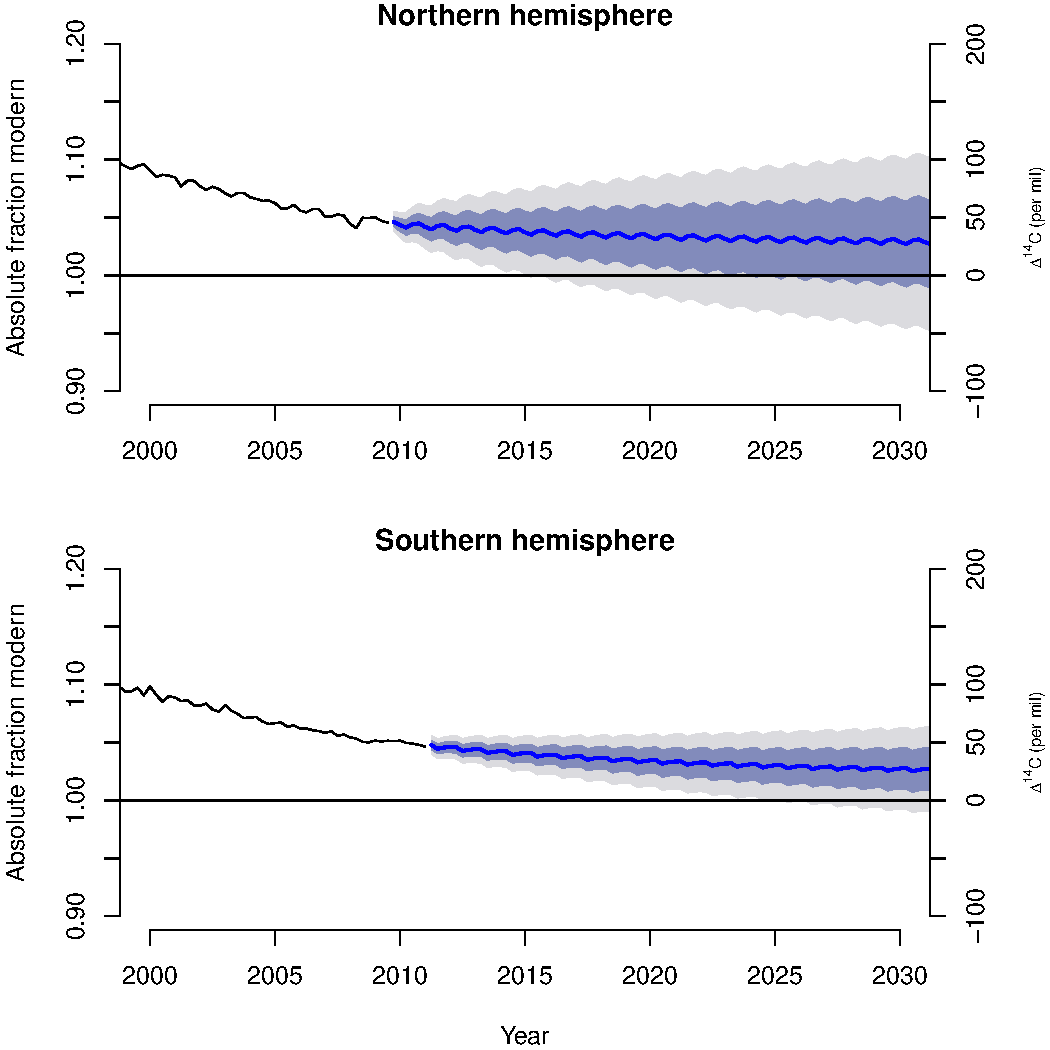
\includegraphics[scale=0.7]{Figures/Forecast} % requires the graphicx package
%   \caption{Forecast of atmospheric radiocarbon for the northern and southern hemispheres based on the best ETS model. Shaded regions in gray and blue show the 95 and 80\% prediction intervals. }
%   \label{fig:Forecast}
%\end{figure}

To predict the decline in atmospheric radiocarbon for central Europe based on the Jungfraujoch and Schauinsland stations, I ran a forecast selecting the ETS model that best matches the observations reported in \citet{Levin2013Tellus} (Figure \ref{fig:ForecastEurope}b). In this forecast, the rate of radiocarbon decline is faster, and mean atmospheric radiocarbon crosses the $\Delta^{14}$C = 0 $\permil$ threshold much earlier.

%\begin{figure}[htbp]
%   \centering
%   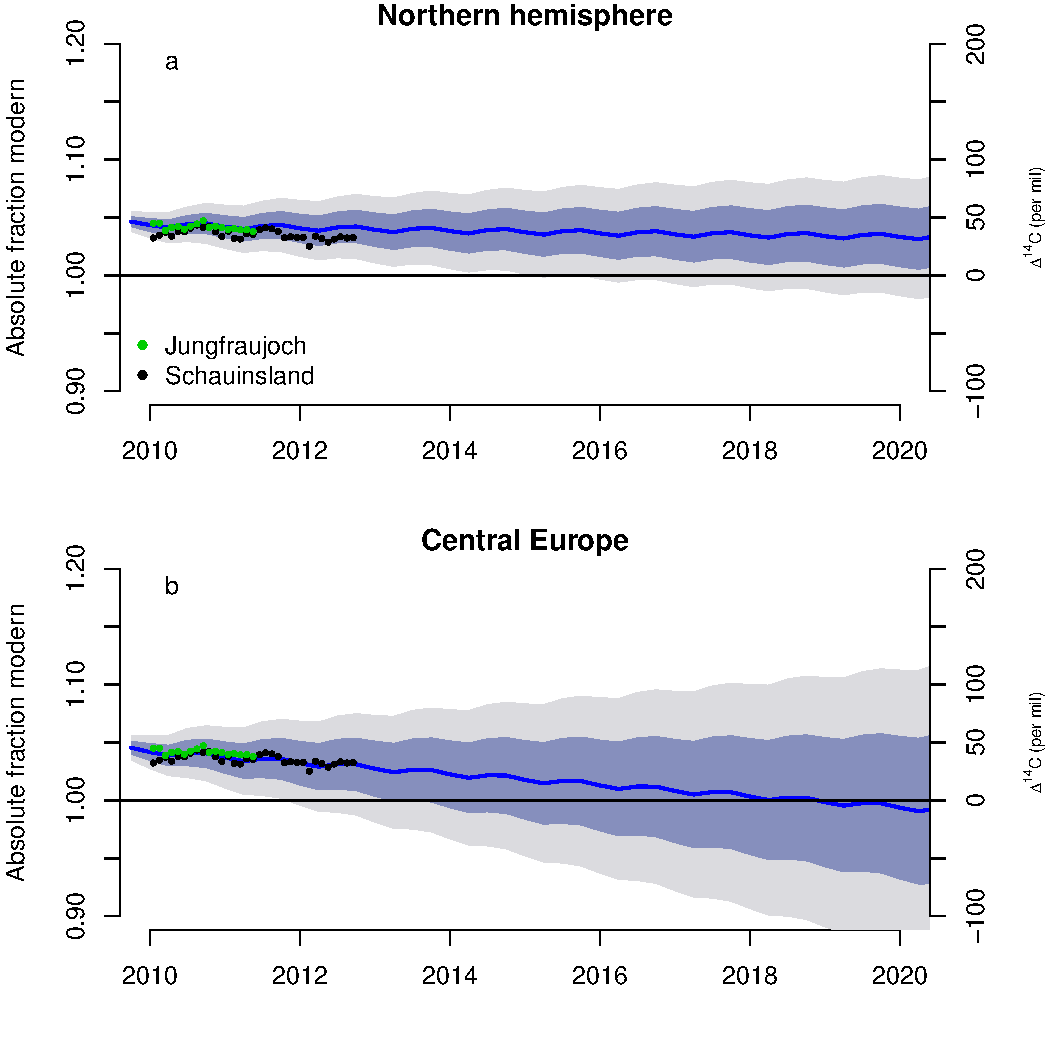
\includegraphics[scale=0.7]{Figures/ForecastEurope} % requires the graphicx package
%   \caption{a) Forecast (with 80 and 95\% prediction intervals) for the northern hemisphere radiocarbon curve compared to observations at the Jungfraujoch and Schauinsland reported in \citet{Levin2013Tellus}. b) Optimized forecast for central Europe forcing the model to pass through the observations from these two stations.}
%   \label{fig:ForecastEurope}
%\end{figure}

Atmospheric radiocarbon is expected to return to pre-1950s levels within the next decades with different probabilities for the different hemispheres. Values of $\Delta^{14}$C $\leq 0 \permil$ are within 95\% prediction intervals of the forecast starting as early as 2016 for the northern hemisphere, and 2025 for the southern hemisphere. For central Europe, it is very likely ($> 90$\% probability) that the $\Delta^{14}$C $\leq 0 \permil$ threshold is being crossed by summer 2018.


%\begin{figure}[htbp]
%   \centering
%   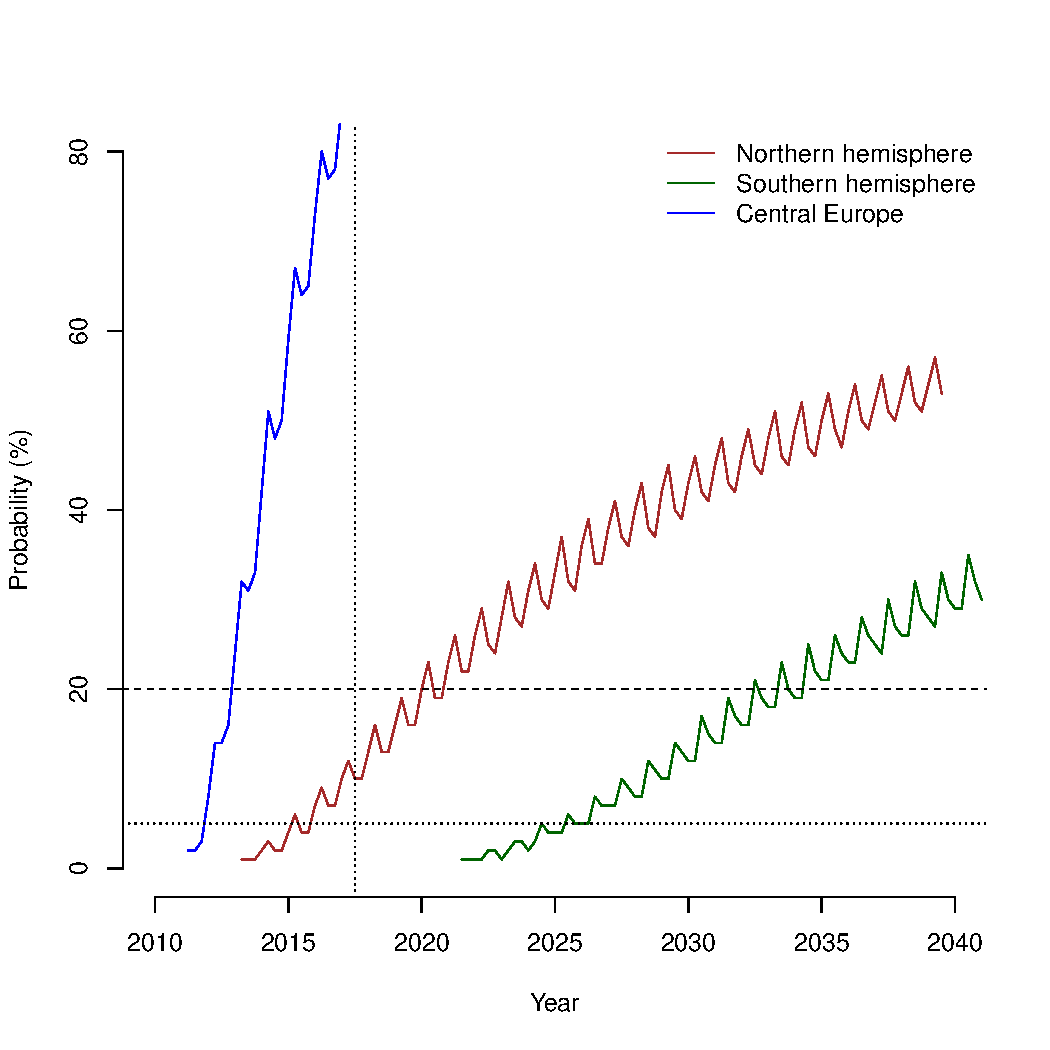
\includegraphics[scale=0.7]{Figures/Prob} % requires the graphicx package
%   \caption{Probability of $\Delta^{14}$C $\leq 0 \permil$ for the different hemispheric zones calculated as 100 minus different probability levels of the lower prediction interval for each forecast time. As a reference, 20 and 5\% probability levels are presented in dashed and dotted lines, respectively.}
%   \label{fig:Prob}
%\end{figure}

Although the hemispheric averages of background air are expected to return to pre-1950 levels within the next decades, this threshold has been already crossed locally in major cities around the world (Figure \ref{fig:Cities}, Table \ref{tab:cities}). Air in metropolitan areas with high fossil-fuel emission levels such as Medell\'in, Stockholm, and the Newport Beach area in California show the highest influence of fossil-fuel derived carbon. 
Air in European cities such as Berlin and Prague had not crossed the pre-1950 level yet, but Jerusalem was in the limit in 2014 ($-0.1 \pm 2.4$ \permil). As expected, the high altitude samples from the Austrian Alps are very close to the forecasted global values, whereas the samples from Rocky Mountain National Park were much below the forecasted global average, but within the 95\% prediction interval of the forecast.

%\begin{figure}[htbp]
%   \centering
%   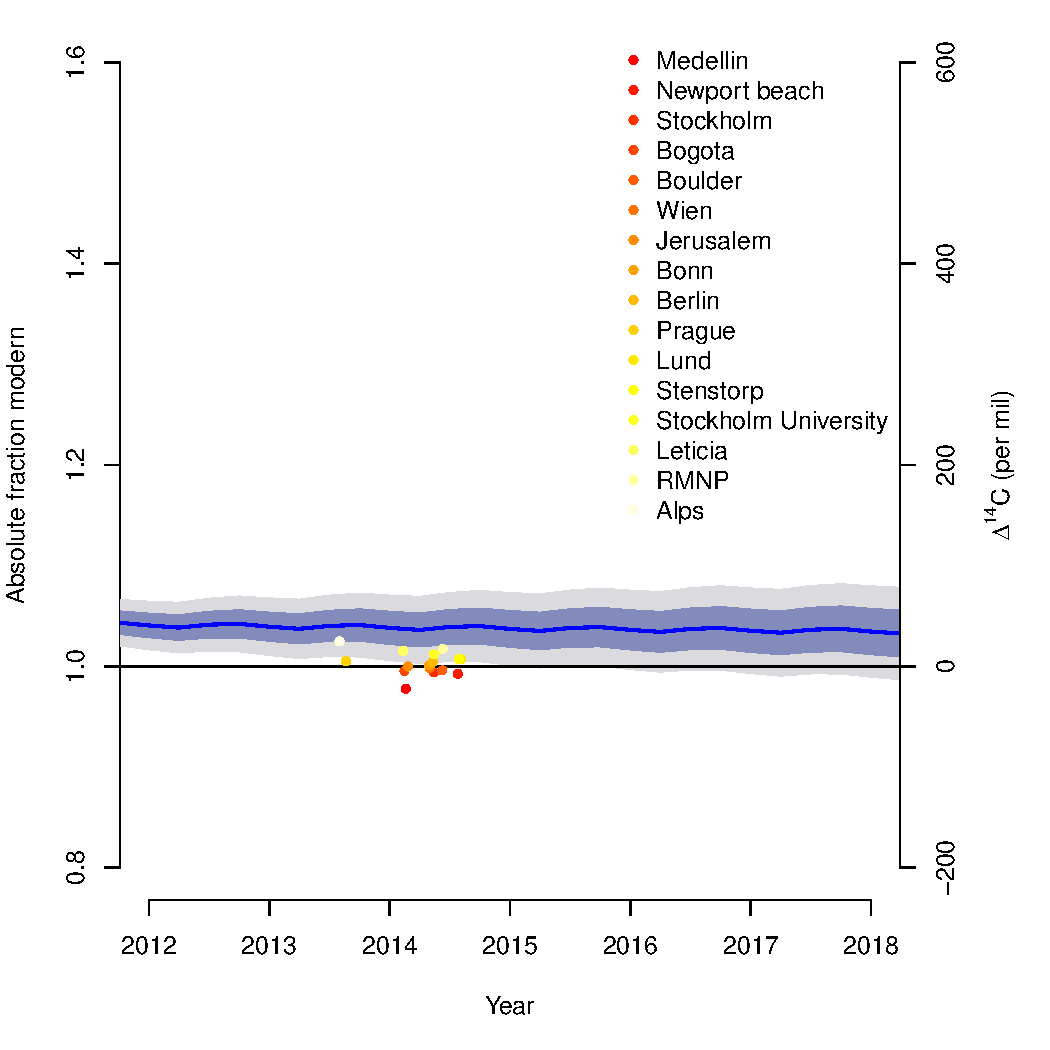
\includegraphics[scale=0.7]{Figures/Cities} % requires the graphicx package
%   \caption{Forecasted northern hemisphere atmospheric radiocarbon concentrations (with 80 and 95\% prediction intervals), based on data from \citet{Hua2013Radiocarbon}, superimposed with radiocarbon concentration measured in plants growing on different industrial cities and remote areas without fossil fuel influence. This radiocarbon concentration represents the mix of fossil-fuel derived carbon and the mixing with background air. }
%   \label{fig:Cities}
%\end{figure}


\section{Discussion}
The time series decomposition presented here shows properties of the trend, slope, and seasonality of atmospheric radiocarbon for different hemispheric zones that complements previous analyses based on sets of individual stations \citep{Levin2010Tellus, Graven2012JGR, Levin2013Tellus} and global carbon models \citep{Caldeira1998GRL, Randerson2002GBC, Turnbull2009JGR, Levin2010Tellus, Graven2015PNAS}. One main advantage of this analysis is the use of the harmonized series compiled by \citet{Hua2013Radiocarbon}, which provide a spatial average across the different stations from which atmospheric radiocarbon has been measured. The series also resolve issues of temporal gaps for the individual stations, and give a comprehensive overview of the dynamic behavior of atmospheric radiocarbon in background air during the past 40 years for the two hemispheres. 

The series decomposition analyses showed that the overall decline of atmospheric radiocarbon was higher in the northern hemisphere than in the southern hemisphere. This is not surprising because the large levels of fossil-fuel emissions in the northern hemisphere are expected to significantly dilute atmospheric radiocarbon \citep{Levin1989Radiocarbon, Levin2010Tellus, Turnbull2009JGR, Graven2012JGR}. Rates of decline since 2005 have been below $ -5 \permil$ per year. This implies that if rates of decline continue decreasing, they may pose significant challenges for detecting annual trends in atmospheric radiocarbon given that the uncertainty in new generation AMS systems is between 3 to 2$\permil$ \citep{Synal2007, Wacker2010}.

Atmospheric radiocarbon is expected to return to pre-1950 levels in the northern hemisphere by 2020, the year predicted by  \citet{Caldeira1998GRL}, with a probability $\sim$20\% (Figure \ref{fig:Prob}). In the southern hemisphere however, it is unlikely that atmospheric radiocarbon reach values below 0 $\permil$ by 2020. Based on more recent observations from central Europe, the pre-1950 threshold may be crossed with high probability ($>$90\%) by summer 2018 (Figure \ref{fig:Prob}). 

It is not possible to attribute any particular process that may contribute to the observed trends in the data with this statistical approach. However, previous analyses \citep{Caldeira1998GRL, Randerson2002GBC, Levin2013Tellus, Currie2011} may help to explain some of the properties of the observed time series. For instance, different processes are responsible for determining atmospheric radiocarbon content: fossil fuel emissions, ocean-atmosphere exchange, stratosphere-troposphere mixing, terrestrial ecosystem fluxes, emissions from nuclear industry, and cosmogenic production \citep{Oeschger1975Tellus, Randerson2002GBC, Naegler2006, Levin2010Tellus, Graven2015PNAS}. The recent slower rates of decline in the northern hemisphere may be explained by the contribution of the terrestrial biosphere and oceans that return decades-old bomb radiocarbon and therefore counterbalance the effect of increased fossil fuel emissions \citep{Caldeira1998GRL, Randerson2002GBC, Currie2011}. For the southern hemisphere, ocean-atmosphere exchange plays a larger role, and the slow in radiocarbon decline in recent years may be explained by return of bomb radiocarbon by the mixed layer \citep{Currie2011}.

The combined effect of terrestrial biosphere, ocean exchange, fossil-fuel emissions as well as horizontal and vertical air transport may have an important contribution in reducing the amplitude of the seasonal cycle \citep{Levin2010Tellus}. The best ETS model identified here predicts the seasonal cycle as proportional to the trend term; i.e. the higher the amount of radiocarbon in the atmosphere the higher the amplitude of the seasonal cycle, and as radiocarbon content decline in both hemispheres so does its seasonality. Given that the growth term of the series had stabilized in the recent decade, the amplitude of the seasonal cycle had remained constant in the last part of the curve. These results are consistent with model predictions by \citet{Randerson2002GBC}, who predicted a decline in seasonality over time due to decrease in seasonality in ocean and terrestrial biosphere exchange, with strong contributions from fossil-fuel signals. 


\citet{Caldeira1998GRL}, and more recently \citet{Graven2015PNAS}, predicted that in a business-as-usual scenario of fossil-fuel emissions, radiocarbon content would return to pre-1950 levels by $\sim$2020. Current trajectories of atmospheric radiocarbon seem to agree with this prediction, but with important differences among hemispheric regions. The $\Delta^{14}$C $\leq 0 \permil$ threshold would be crossed in the northern hemisphere with higher probability than in the southern hemisphere, which may be a consequence of differences in contributions between the terrestrial biosphere and the oceans, the later being more relevant for the southern hemisphere. 
It is also likely that the rate of decline of atmospheric radiocarbon in the northern hemisphere may increase in the future (become more negative) if the previously sequestered bomb-radiocarbon is exhausted, and then fossil-fuel derived carbon may have a larger influence in the northern hemisphere. This is clearly illustrated in the urban areas we analyzed where fossil-fuel emissions dominate over terrestrial exchange  and therefore radiocarbon is close or have already crossed the $\Delta^{14}$C $\leq 0 \permil$ threshold. 

The forecasted atmospheric radiocarbon curves presented here may be useful for different studies where data on the atmospheric background is not available after the latest release of the compiled curves \citep{Hua2013Radiocarbon}. The methodology of time-series decomposition and forecast may also be useful to produce forecasts for individual stations or for new releases of compiled curves. However, care must be taken in using these forecasts in different applications, and prediction uncertainties must always be considered.
Possible changes in the rates of decline of atmospheric radiocarbon for the different hemispheres may deviate in the future from the rates calculated in the time-series decomposition presented here. Therefore, these forecasted radiocarbon trends must be used with caution.


\section*{Acknowledgements}
Funding was provided by the Max Planck Society and the German Research Foundation through the Emmy-Noether programme (SI 1953/2-1).

\newpage

%\bibliography{../../Bibliography/TEE,c14refs}
%\bibliographystyle{apalike}
\begin{thebibliography}{}

\bibitem[Athanasopoulos et~al., 2017]{Athanasopoulos}
Athanasopoulos, G., Hyndman, R.~J., Kourentzes, N., and Petropoulos, F. (2017).
\newblock Forecasting with temporal hierarchies.
\newblock {\em European Journal of Operational Research}, 262(1):60 -- 74.

\bibitem[Berger et~al., 1987]{Berger1987}
Berger, R., Jackson, T.~B., Michael, R., and Suess, H.~E. (1987).
\newblock Radiocarbon content of tropospheric {CO$_2$ at China Lake,
  California} 1977--1983.
\newblock {\em Radiocarbon}, 29(1):18--23.

\bibitem[Caldeira et~al., 1998]{Caldeira1998GRL}
Caldeira, K., Rau, G.~H., and Duffy, P.~B. (1998).
\newblock Predicted net efflux of radiocarbon from the ocean and increase in
  atmospheric radiocarbon content.
\newblock {\em Geophysical Research Letters}, 25(20):3811--3814.

\bibitem[Cleveland et~al., 1983]{Cleveland1983}
Cleveland, W.~S., Freeny, A.~E., and Graedel, T.~E. (1983).
\newblock The seasonal component of atmospheric {CO$_2$}: Information from new
  approaches to the decomposition of seasonal time series.
\newblock {\em Journal of Geophysical Research: Oceans}, 88(C15):10934--10946.

\bibitem[Currie et~al., 2011]{Currie2011}
Currie, K.~I., Brailsford, G., Nichol, S., Gomez, A., Sparks, R., Lassey,
  K.~R., and Riedel, K. (2011).
\newblock Tropospheric {$^{14}$CO$_2$} at wellington, new zealand: the world's
  longest record.
\newblock {\em Biogeochemistry}, 104(1):5--22.

\bibitem[Graven, 2015]{Graven2015PNAS}
Graven, H.~D. (2015).
\newblock Impact of fossil fuel emissions on atmospheric radiocarbon and
  various applications of radiocarbon over this century.
\newblock {\em Proceedings of the National Academy of Sciences},
  112(31):9542--9545.

\bibitem[Graven et~al., 2012]{Graven2012JGR}
Graven, H.~D., Guilderson, T.~P., and Keeling, R.~F. (2012).
\newblock Observations of radiocarbon in {CO$_2$} at seven global sampling
  sites in the {Scripps} flask network: Analysis of spatial gradients and
  seasonal cycles.
\newblock {\em Journal of Geophysical Research: Atmospheres}, 117(D2).
\newblock D02303.

\bibitem[Hertelendi and Csongor, 1983]{Hertelendi1983}
Hertelendi, E. and Csongor, E. (1983).
\newblock Anthropogenic 14 c excess in the troposphere between 1951 and 1978
  measured in tree rings.
\newblock {\em Radiochemical and Radioanalytical letters}, 56(2):103--110.

\bibitem[Hsueh et~al., 2007]{Hsueh2007GRL}
Hsueh, D.~Y., Krakauer, N.~Y., Randerson, J.~T., Xu, X., Trumbore, S.~E., and
  Southon, J.~R. (2007).
\newblock Regional patterns of radiocarbon and fossil fuel-derived {CO2} in
  surface air across {North America}.
\newblock {\em Geophysical Research Letters}, 34(2):n/a--n/a.
\newblock L02816.

\bibitem[Hua and Barbetti, 2004]{Hua2004}
Hua, Q. and Barbetti, M. (2004).
\newblock Review of tropospheric bomb 14c data for carbon cycle modeling and
  age calibration purposes.
\newblock {\em Radiocarbon}, 46(3):1273--1298.

\bibitem[Hua et~al., 2000]{Hua2000}
Hua, Q., Barbetti, M., Jacobsen, G., Zoppi, U., and Lawson, E. (2000).
\newblock {Bomb radiocarbon in annual tree rings from Thailand and Australia}.
\newblock {\em Nuclear Instruments and Methods in Physics Research Section B:
  Beam Interactions with Materials and Atoms}, 172(1):359 -- 365.
\newblock 8th International Conference on Accelerator Mass Spectrometry.

\bibitem[Hua et~al., 2012]{Hua2012GRL}
Hua, Q., Barbetti, M., Levchenko, V.~A., D'Arrigo, R.~D., Buckley, B.~M., and
  Smith, A.~M. (2012).
\newblock Monsoonal influence on southern hemisphere {$^{14}$CO$_2$}.
\newblock {\em Geophysical Research Letters}, 39(19).
\newblock L19806.

\bibitem[Hua et~al., 2013]{Hua2013Radiocarbon}
Hua, Q., Barbetti, M., and Rakowski, A. (2013).
\newblock Atmospheric radiocarbon for the period 1950--2010.
\newblock {\em Radiocarbon}, 55(4):2059--2072.

\bibitem[Hyndman et~al., 2008]{Hyndman2008}
Hyndman, A.~R., Koehler, A., Ord, K., and Snyder, R. (2008).
\newblock {\em Forecasting with Exponential Smoothing}.
\newblock Springer Series in Statistics. Springer Berlin Heidelberg.

\bibitem[Hyndman and Khandakar, 2008]{Hyndman2008JSS}
Hyndman, R.~J. and Khandakar, Y. (2008).
\newblock Automatic time series forecasting: The forecast package for {R}.
\newblock {\em Journal of Statistical Software}, 27(3):1--22.

\bibitem[Levin and Kromer, 1997]{Levin1997}
Levin, I. and Kromer, B. (1997).
\newblock Twenty years of atmospheric {$^{14}$CO$_2$} observations at
  {Schauinsland station, Germany}.
\newblock {\em Radiocarbon}, 39(2):205--218.

\bibitem[Levin and Kromer, 2004]{Levin2004}
Levin, I. and Kromer, B. (2004).
\newblock The tropospheric {$^{14}$CO$_2$} level in mid-latitudes of the
  northern hemisphere (1959--2003).
\newblock {\em Radiocarbon}, 46(3):1261--1272.

\bibitem[Levin et~al., 2013]{Levin2013Tellus}
Levin, I., Kromer, B., and Hammer, S. (2013).
\newblock Atmospheric {$\Delta^{14}$CO2} trend in {Western European} background
  air from 2000 to 2012.
\newblock {\em Tellus B}, 65(0).

\bibitem[Levin et~al., 2010]{Levin2010Tellus}
Levin, I., Naegler, T., Kromer, B., Diehl, M., Francey, R.~J., Gomez-Pelaez,
  A.~J., Steele, L.~P., Wagenbach, D., Weller, R., and Worthy, D.~E. (2010).
\newblock Observations and modelling of the global distribution and long-term
  trend of atmospheric 14co2.
\newblock {\em Tellus B}, 62(1):26--46.

\bibitem[Levin et~al., 1989]{Levin1989Radiocarbon}
Levin, I., Schuchard, J., Kromer, B., and Muennich, K. (1989).
\newblock The continental {European Suess} effect.
\newblock {\em Radiocarbon}, 31(3):431--440.

\bibitem[Manning et~al., 1990]{Manning1990}
Manning, M.~R., Lowe, D.~C., Melhuish, W.~H., Sparks, R.~J., Wallace, G.,
  Brenninkmeijer, C. A.~M., and McGill, R.~C. (1990).
\newblock The use of radiocarbon measurements in atmospheric studies.
\newblock {\em Radiocarbon}, 32(1):37--58.

\bibitem[Meijer et~al., 2006]{Meijer2006}
Meijer, H. A.~J., Pertuisot, M.~H., and van~der Plicht, J. (2006).
\newblock High-accuracy {$^{14}$C} measurements for atmospheric {CO$_2$}
  samples by {AMS}.
\newblock {\em Radiocarbon}, 48(3):355--372.

\bibitem[Naegler and Levin, 2006]{Naegler2006}
Naegler, T. and Levin, I. (2006).
\newblock Closing the global radiocarbon budget 1945--2005.
\newblock {\em Journal of Geophysical Research: Atmospheres},
  111(D12):n/a--n/a.
\newblock D12311.

\bibitem[Nijman and Palm, 1990]{Nijman1990}
Nijman, T.~E. and Palm, F.~C. (1990).
\newblock Predictive accuracy gain from disaggregate sampling in {ARIMA}
  models.
\newblock {\em Journal of Business \& Economic Statistics}, 8(4):405--415.

\bibitem[Nydal and Loevseth, 1996]{Nydal1996}
Nydal, R. and Loevseth, K. (1996).
\newblock {\em Carbon-14 Measurements in Atmospheric {CO$_2$} from Northern and
  Southern Hemisphere Sites, 1962-1993}.
\newblock Oak Ridge National Laboratory.

\bibitem[Oeschger et~al., 1975]{Oeschger1975Tellus}
Oeschger, H., Siegenthaler, U., Schotterer, U., and Gugelmann, A. (1975).
\newblock A box diffusion model to study the carbon dioxide exchange in nature.
\newblock {\em Tellus}, 27(2):168--192.

\bibitem[Park et~al., 2002]{Park2002}
Park, J.~H., Kim, J.~C., Cheoun, M.~K., Kim, I.~C., Youn, M., Liu, Y.~H., and
  Kim, E.~S. (2002).
\newblock {14C level at Mt Chiak and Mt Kyeryong in Korea}.
\newblock {\em Radiocarbon}, 44(2):559--566.

\bibitem[Rakowski et~al., 2013]{Rakowski2013}
Rakowski, A.~Z., Nadeau, M.-J., Nakamura, T., Pazdur, A., Pawe{\l}czyk, S., and
  Piotrowska, N. (2013).
\newblock Radiocarbon method in environmental monitoring of {CO$_2$} emission.
\newblock {\em Nuclear Instruments and Methods in Physics Research Section B:
  Beam Interactions with Materials and Atoms}, 294:503 -- 507.
\newblock Proceedings of the Twelfth International Conference on Accelerator
  Mass Spectrometry, Wellington, New Zealand, 20-25 March 2011.

\bibitem[Randerson et~al., 2002]{Randerson2002GBC}
Randerson, J.~T., Enting, I.~G., Schuur, E. A.~G., Caldeira, K., and Fung,
  I.~Y. (2002).
\newblock Seasonal and latitudinal variability of troposphere
  {$\Delta^{14}$CO$_2$}: Post bomb contributions from fossil fuels, oceans, the
  stratosphere, and the terrestrial biosphere.
\newblock {\em Global Biogeochemical Cycles}, 16(4):59--1--59--19.

\bibitem[Rossana and Seater, 1995]{Rossana1995}
Rossana, R.~J. and Seater, J.~J. (1995).
\newblock Temporal aggregation and economic time series.
\newblock {\em Journal of Business \& Economic Statistics}, 13(4):441--451.

\bibitem[Sierra et~al., 2014]{SierraGMD14}
Sierra, C.~A., M\"uller, M., and Trumbore, S.~E. (2014).
\newblock Modeling radiocarbon dynamics in soils: {SoilR} , version 1.1.
\newblock {\em Geosci. Model Dev.}, 7(7):1919--1931.
\newblock GMD.

\bibitem[Steinhof et~al., 2004]{Steinhof2004Radiocarbon}
Steinhof, A., Adamiec, G., Gleixner, G., Wagner, T., and van Klinken, G.
  (2004).
\newblock The new {$^{14}$C} analysis laboratory in {Jena, Germany}.
\newblock {\em Radiocarbon}, 46(1):51--58.

\bibitem[Suess, 1953]{Suess1953}
Suess, H.~E. (1953).
\newblock Natural radiocarbon and the rate of exchange of carbon dioxide
  between the atmosphere and the sea.
\newblock In {\em Nuclear Processes in Geological Settings}, pages 52--56.
  National Research Council Publications.

\bibitem[Suess, 1955]{Suess1955Sci}
Suess, H.~E. (1955).
\newblock Radiocarbon concentration in modern wood.
\newblock {\em Science}, 122(3166):415--417.

\bibitem[Synal et~al., 2007]{Synal2007}
Synal, H.-A., Stocker, M., and Suter, M. (2007).
\newblock {MICADAS: A new compact radiocarbon AMS system}.
\newblock {\em Nuclear Instruments and Methods in Physics Research Section B:
  Beam Interactions with Materials and Atoms}, 259(1):7 -- 13.
\newblock Accelerator Mass Spectrometry.

\bibitem[Tans et~al., 1979]{Tans1979Nature}
Tans, P.~P., de~Jong, A. F.~M., and Mook, W.~G. (1979).
\newblock Natural atmospheric {14C} variation and the {Suess} effect.
\newblock {\em Nature}, 280(5725):826--828.

\bibitem[Trumbore et~al., 2016]{Trumbore2016}
Trumbore, S.~E., Sierra, C.~A., and Hicks~Pries, C.~E. (2016).
\newblock Radiocarbon nomenclature, theory, models, and interpretation:
  Measuring age, determining cycling rates, and tracing source pools.
\newblock In Schuur, A.~E., Druffel, E., and Trumbore, E.~S., editors, {\em
  Radiocarbon and Climate Change: Mechanisms, Applications and Laboratory
  Techniques}, pages 45--82. Springer International Publishing.

\bibitem[Turnbull et~al., 2009]{Turnbull2009JGR}
Turnbull, J., Rayner, P., Miller, J., Naegler, T., Ciais, P., and Cozic, A.
  (2009).
\newblock On the use of {$^{14}$CO$_2$} as a tracer for fossil fuel {CO$_2$}:
  Quantifying uncertainties using an atmospheric transport model.
\newblock {\em Journal of Geophysical Research: Atmospheres}, 114(D22).
\newblock D22302.

\bibitem[Turnbull et~al., 2007]{Turnbull2007}
Turnbull, J.~C., Lehman, S.~J., Miller, J.~B., Sparks, R.~J., Southon, J.~R.,
  and Tans, P.~P. (2007).
\newblock A new high precision {$^{14}$CO$_2$} time series for {North American}
  continental air.
\newblock {\em Journal of Geophysical Research: Atmospheres}, 112(D11).
\newblock D11310.

\bibitem[Vogel and Marais, 1971]{Vogel1971}
Vogel, J.~C. and Marais, M. (1971).
\newblock Pretoria radiocarbon dates i.
\newblock {\em Radiocarbon}, 13(2):378--394.

\bibitem[Wacker et~al., 2010]{Wacker2010}
Wacker, L., Bonani, G., Friedrich, M., Hajdas, I., Kromer, B., N{\v e}mec, M.,
  Ruff, M., Suter, M., Synal, H.-A., and Vockenhuber, C. (2010).
\newblock Micadas: Routine and high-precision radiocarbon dating.
\newblock {\em Radiocarbon}, 52(2):252--262.

\bibitem[Yamada et~al., 2005]{Yamada2005}
Yamada, Y., Yasuike, K., and Komura, K. (2005).
\newblock Temporal variation of carbon-14 concentration in tree-ring cellulose
  for the recent 50 years.
\newblock {\em Journal of Nuclear and Radiochemical Sciences}, 6(2):135--138.

\end{thebibliography}


\clearpage

\section*{Tables}

\begin{table}[ht]
\centering \small 
\caption{Slopes of the atmospheric radiocarbon curves ($\pm$ residuals $\varepsilon_t$) calculated for the last years of the series using the obtained ETS model. Values in $\Delta^{14}$C (\permil).} \label{tab:slopes}
\begin{tabular}{rcc} 
  \toprule
Year & Northern hemisphere & Southern hemisphere \\ 
  \midrule
2005 & -5.30 $\pm$ 5.73 & -5.16 $\pm$ 5.31 \\ 
  2006 & -4.30 $\pm$ 4.49 & -4.81 $\pm$ 4.36 \\ 
  2007 & -4.56 $\pm$ 6.47 & -4.59 $\pm$ 8.15 \\ 
  2008 & -4.70 $\pm$ 7.13 & -4.25 $\pm$ 4.31 \\ 
  2009 & -1.49$^{\ast} \pm$ 12.93 & -3.69 $\pm$ 6.00 \\ 
  2010 &   & -2.64 $\pm$ 5.60 \\ 
  2011 &   & -0.82$^{\dagger} \pm$ 6.78 \\ 
   \bottomrule
   \multicolumn{3}{l}{$^{\ast}$ Only includes the first 8 months of the year} \\
   \multicolumn{3}{l}{$^{\dagger}$ Only includes the first 3 months of the year}
\end{tabular}
\end{table}


\begin{table}[ht]
\centering \small 
\caption{Radiocarbon measured in annual plants (mostly {\it Taraxacum spp.}) collected across different cities and natural areas. } \label{tab:cities}
\begin{tabular}{rllccccc} 
  \toprule
Lab ID & City & Country & Sampling date & $\Delta^{14}$C (\permil) & sd (\permil) & Lat & Long \\ 
  \midrule
9241 & Medellin & Colombia & 2014-2-18 & -22.20 & 2.40 & 6.23 & -75.60 \\ 
10911 & Newport beach & USA & 2014-7-26 & -7.40 & 4.00 & 33.67 & -117.87 \\ 
10907 & Stockholm & Sweden & 2014-5-14 & -5.90 & 2.80 & 59.35 & 18.06 \\ 
9243 & Bogota & Colombia & 2014-2-14 & -4.50 & 2.40 & 4.62 & -74.07 \\ 
10909 & Boulder & USA & 2014-6-9 & -3.90 & 3.40 & 40.02 & -105.27 \\ 
10905 & Wien & Austria & 2014-5-2 & -1.50 & 2.90 & 48.23 & 16.42 \\ 
9240 & Jerusalem & Israel & 2014-2-25 & -0.10 & 2.40 & 31.77 & 35.22 \\ 
10904 & Bonn & Germany & 2014-4-30 & 1.00 & 2.90 & 50.70 & 7.15 \\ 
10906 & Berlin & Germany & 2014-5-11 & 4.30 & 3.50 & 52.52 & 13.37 \\ 
9244 & Prague & Czech Republic & 2013-8-21 & 5.20 & 2.40 & 50.08 & 14.42 \\ 
10912 & Lund & Sweden & 2014-8-4 & 7.20 & 3.30 & 55.70 & 13.19 \\ 
10913 & Stenstorp & Sweden & 2014-7-29 & 7.20 & 3.50 & 55.91 & 13.44 \\ 
10908 & Stockholm Uni. & Sweden & 2014-5-14 & 11.90 & 3.10 & 59.37 & 18.06 \\ 
9242 & Leticia & Colombia & 2014-2-10 & 15.30 & 2.40 & -4.21 & -69.94 \\ 
10910 & Rocky Mount. & USA & 2014-6-10 & 17.40 & 3.30 & 40.43 & -105.78 \\ 
10914 & Alps & Austria & 2013-8-1 & 24.80 & 3.20 & 47.13 & 11.31 \\ 
   \bottomrule
\end{tabular}
\end{table}
\clearpage

\section*{Figure captions}


%Fig 1.
\begin{figure}[htbp]
   \centering
%   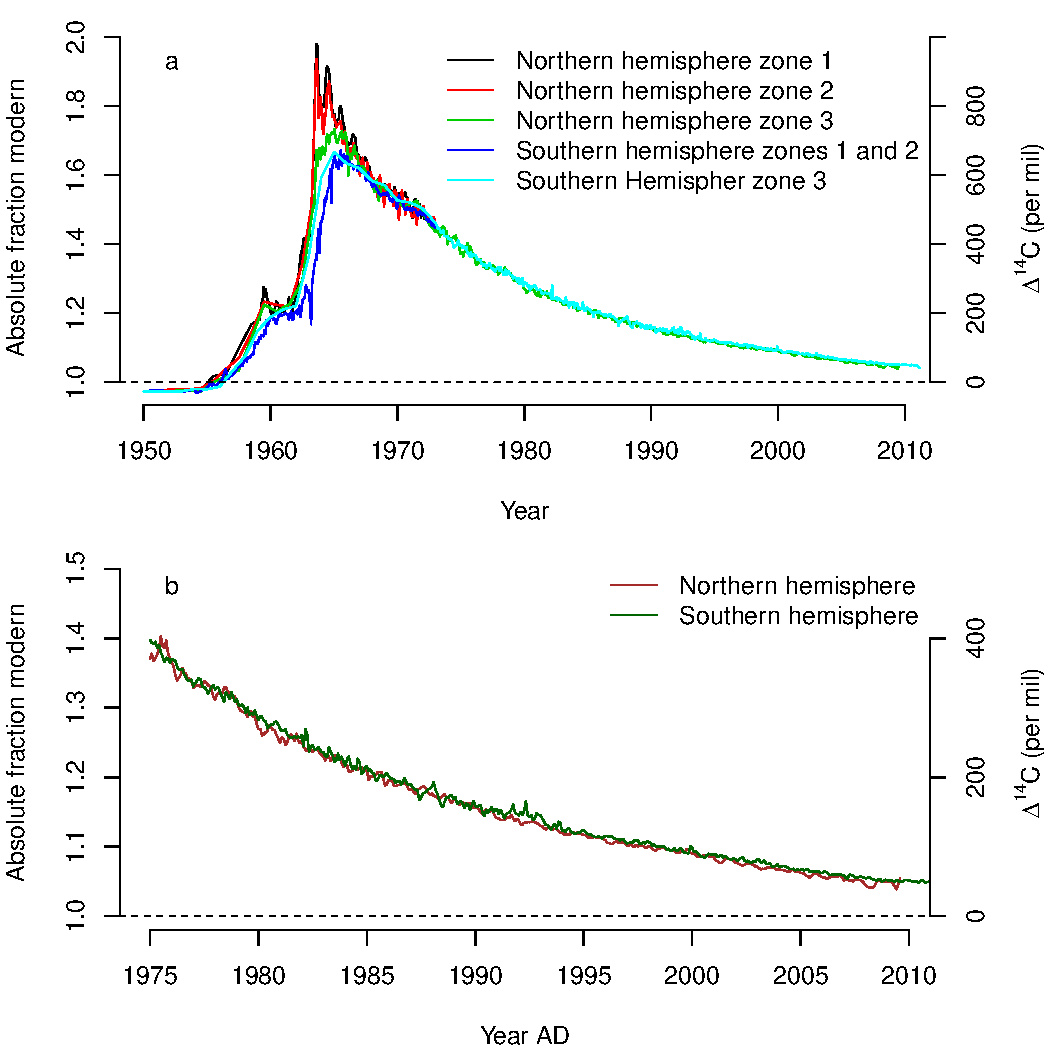
\includegraphics[scale=0.7]{Figures/HuaSeries} % requires the graphicx package
   \caption{Atmospheric radiocarbon curves obtained by \citet{Hua2013Radiocarbon}. a) Original data for four different atmospheric regions, b) time series constructed from original data for the period 1975 to 2010.}
   \label{fig:HuaSeries}
\end{figure}

% Fig 2
\begin{figure}[htbp]
   \centering
%   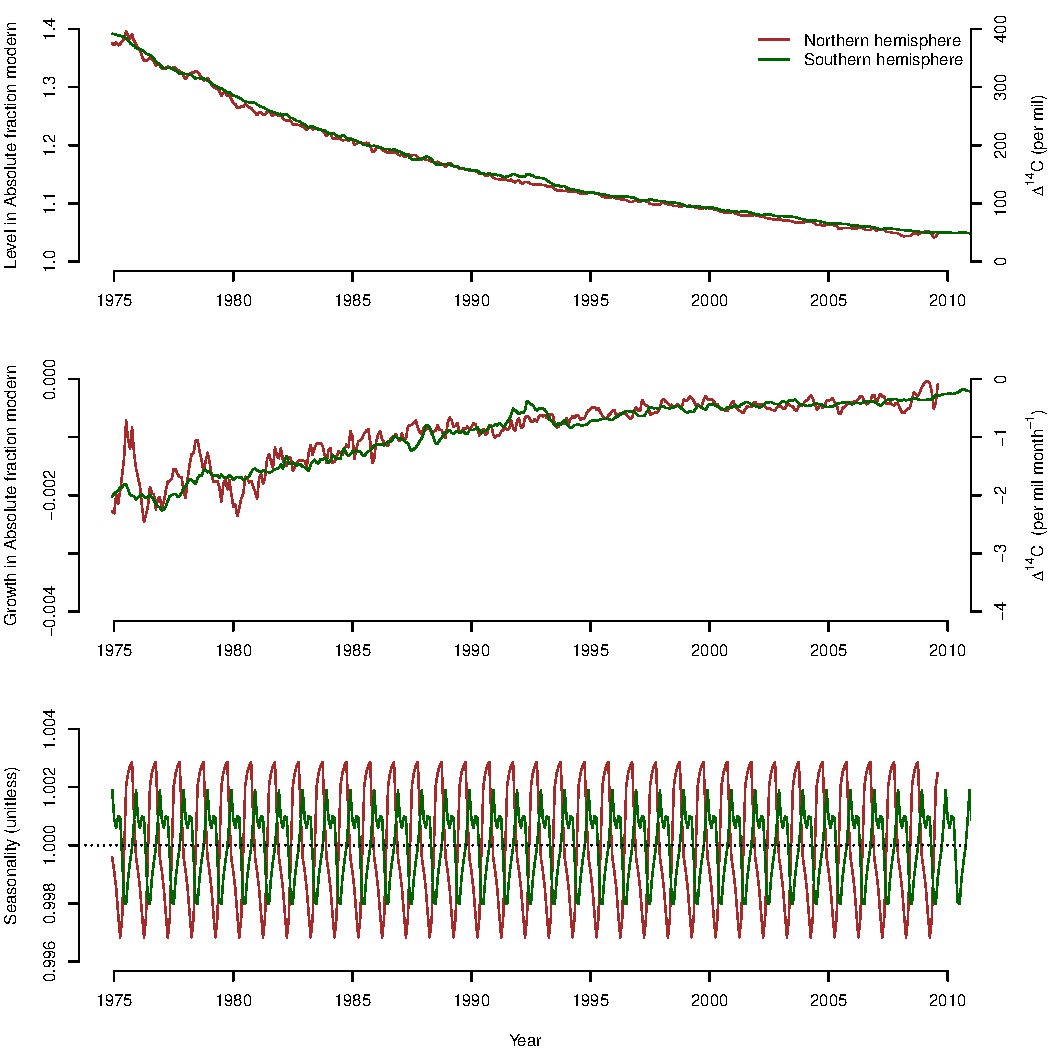
\includegraphics[scale=0.7]{Figures/SlopeSeason} % requires the graphicx package
   \caption{Trend (level and slope) and seasonality of the atmospheric radiocarbon time series predicted by the best-fit model for the hemispheric series compiled by \citet{Hua2013Radiocarbon}. For both series, the best model selected based on the AIC was an ETS model of the form (M,A,M), i.e. a multiplicative term for the error, an additive term for the trend, and a multiplicative term for the seasonality. }
   \label{fig:SlopeSeason}
\end{figure}

% Fig. 3
\begin{figure}[htbp]
   \centering
%   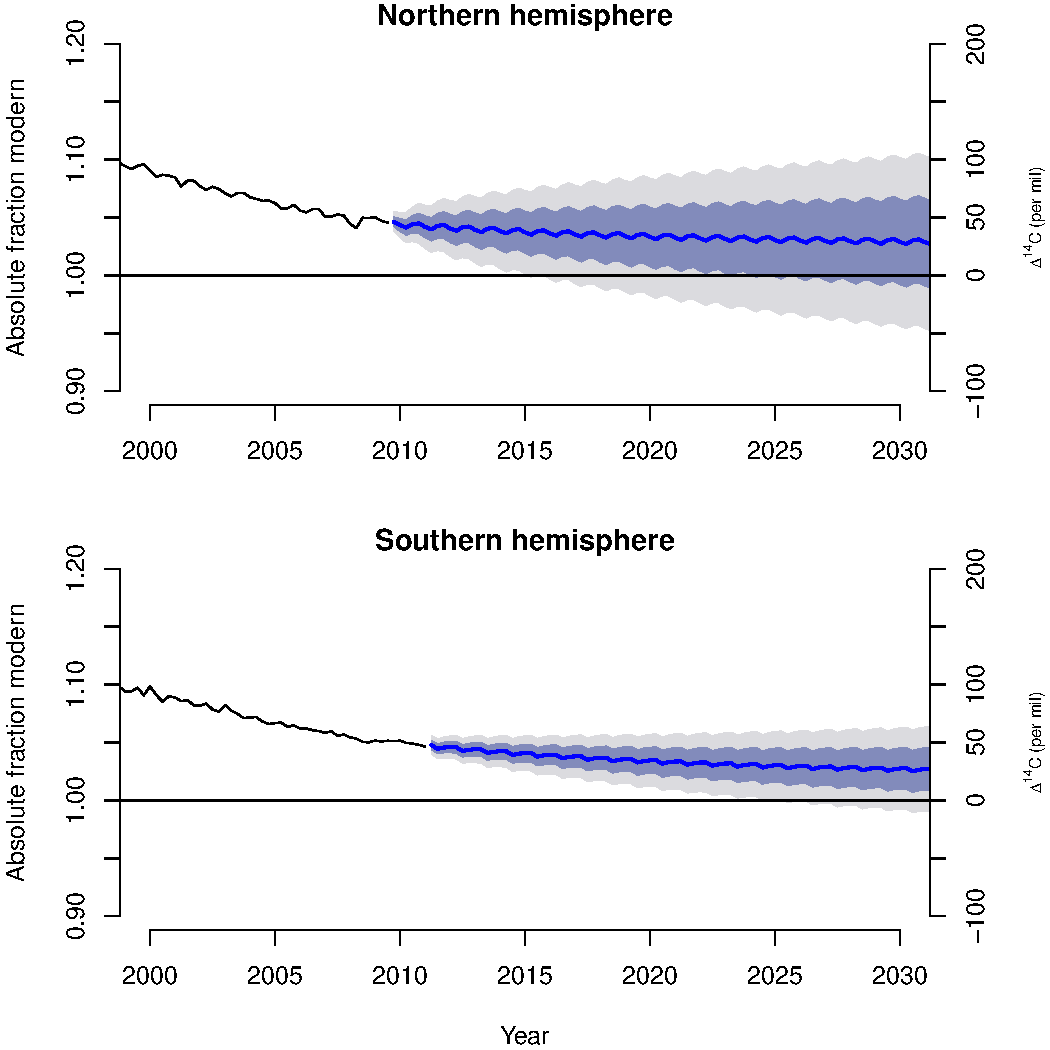
\includegraphics[scale=0.7]{Figures/Forecast} % requires the graphicx package
   \caption{Forecast of atmospheric radiocarbon for the northern and southern hemispheres based on the best ETS model. Shaded regions in gray and blue show the 95 and 68\% prediction intervals. }
   \label{fig:Forecast}
\end{figure}

% Fig 4
\begin{figure}[htbp]
   \centering
%   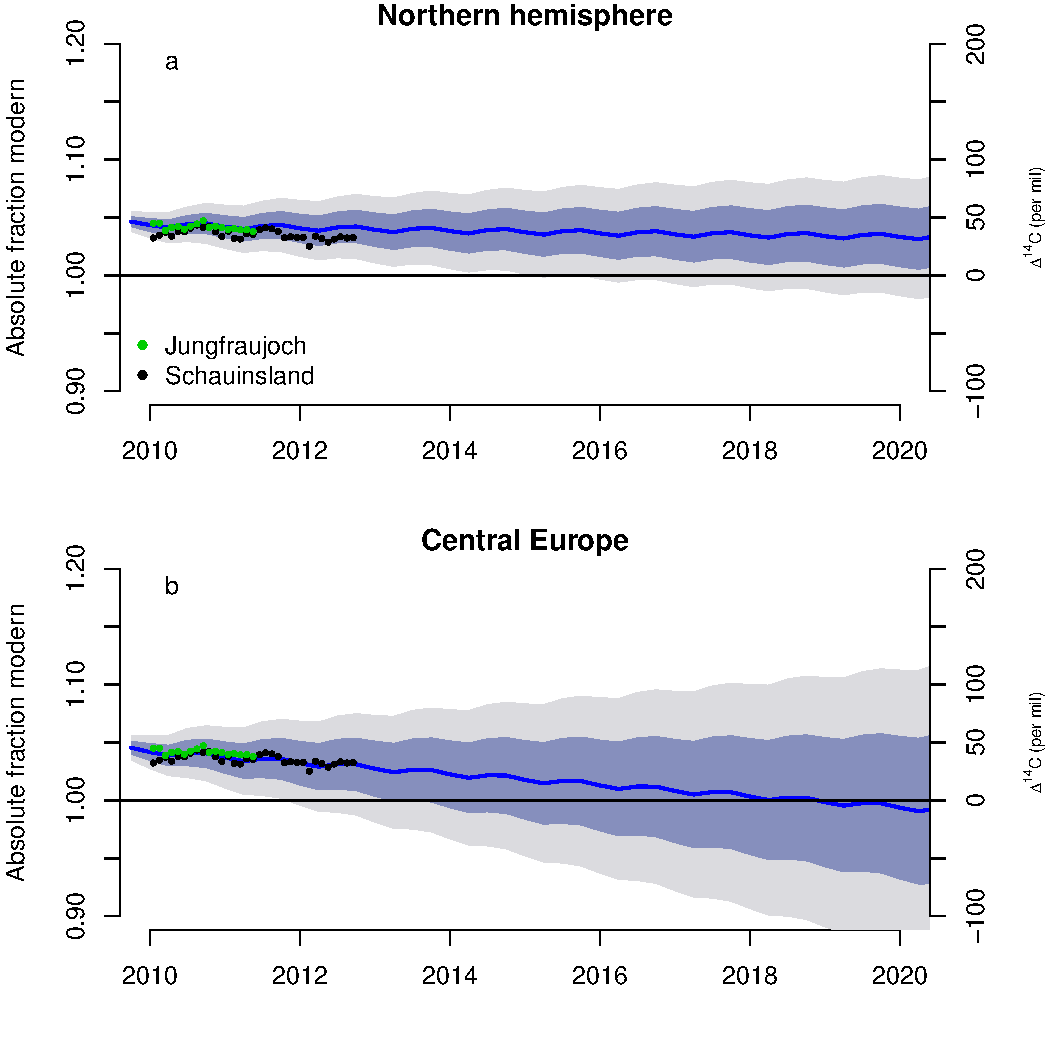
\includegraphics[scale=0.7]{Figures/ForecastEurope} % requires the graphicx package
   \caption{a) Forecast (with 68 and 95\% prediction intervals) for the northern hemisphere radiocarbon curve compared to observations at the Jungfraujoch and Schauinsland reported in \citet{Levin2013Tellus}. b) Optimized forecast for central Europe forcing the model to pass through the observations from these two stations.}
   \label{fig:ForecastEurope}
\end{figure}

% Fig 5

\begin{figure}[htbp]
   \centering
%   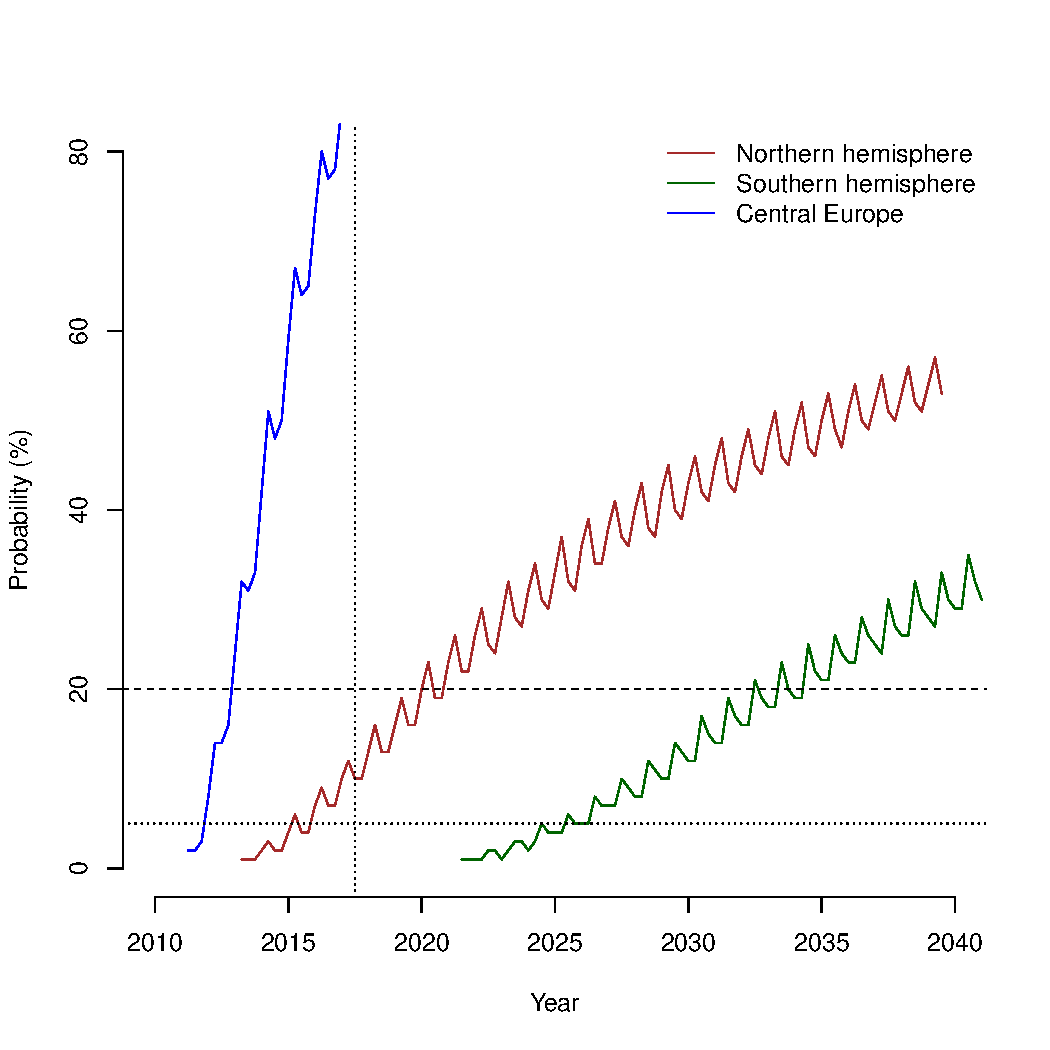
\includegraphics[scale=0.7]{Figures/Prob} % requires the graphicx package
   \caption{Probability of $\Delta^{14}$C $\leq 0 \permil$ for the different hemispheric zones calculated as 100 minus different probability levels of the lower prediction interval for each forecast time. As a reference, 20 and 5\% probability levels are presented in dashed and dotted lines, respectively. The vertical dotted line represents July 2018.}
   \label{fig:Prob}
\end{figure}

% Fig 6
\begin{figure}[htbp]
   \centering
%   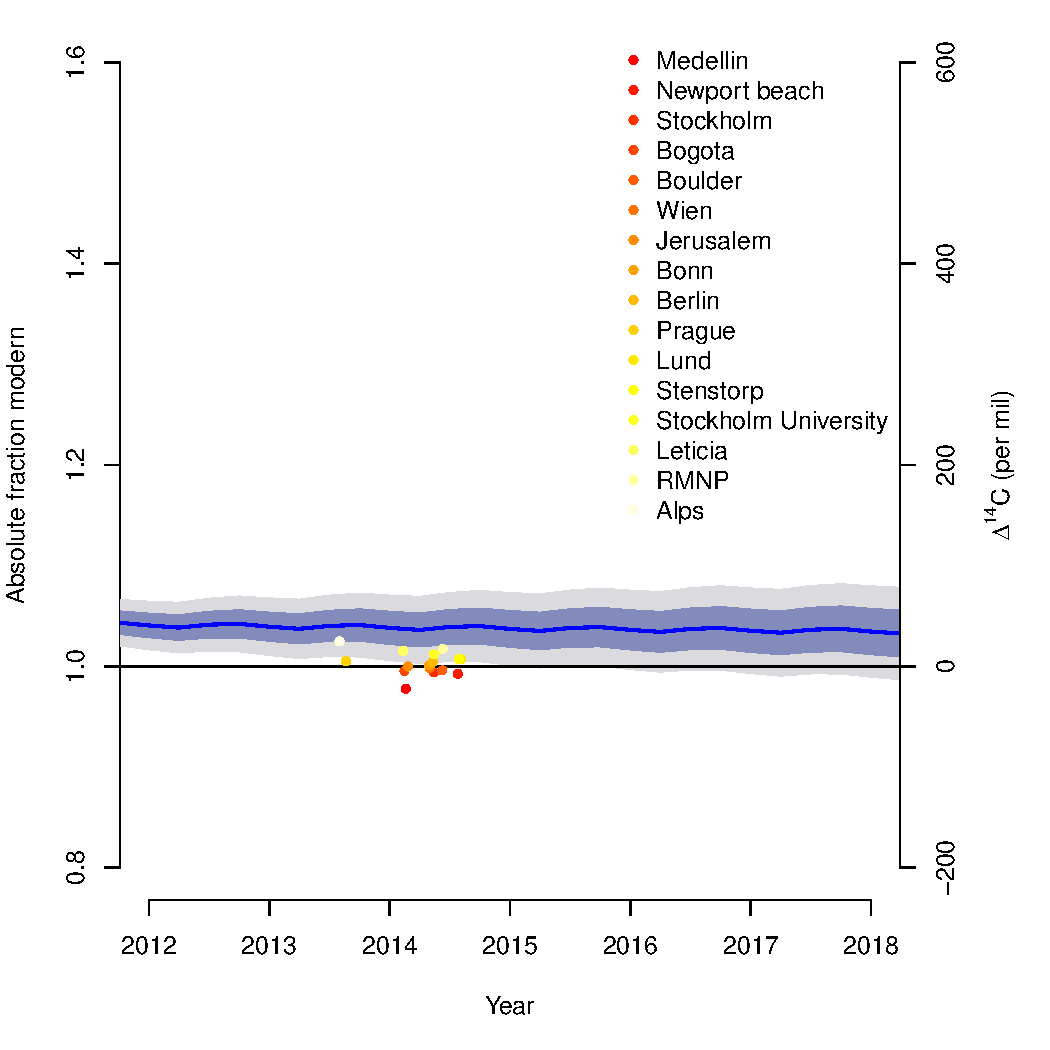
\includegraphics[scale=0.7]{Figures/Cities} % requires the graphicx package
   \caption{Forecasted northern hemisphere atmospheric radiocarbon values (with 68 and 95\% prediction intervals), superimposed with radiocarbon values measured in plants growing on different industrial cities and remote areas without fossil fuel influence. This radiocarbon value represents the mix of fossil-fuel derived carbon and the mixing with background air. }
   \label{fig:Cities}
\end{figure}


\end{document}